In diesem Kapitel werden die Messergebnisse vorgestellt, die eine
Charakterisierung des Lasersystems erlauben. Dabei werden zunächst Messungen
aufgeführt, die die reine Frequenzstabilität der Laser beschreiben. Dazu werden
Lang- und Kurzzeitverhalten sowohl des alten als auch den neuen Lasersystems
untersucht (Abschn. \ref{sec:stabilitaet_der_laser}). Weiterhin wird das
Linearitätsverhalten der \textit{iScans} charakterisiert, wobei die
Nichtlinearitäten und deren Auswirkung auf die
Frequenzverstimmungsroutine gemessen werden (Abschn.
\ref{sec:linearisierung}). Abschnitt \ref{spektroskopie_an_uran} beschäftigt
sich mit den bishereigen spektroskopischen Messungen an Uran mit dem alten und
neuen System, dem bisher verwendeten Anregungsschema und der Suche nach neuen
Anregungsschemata. In Abschn. \ref{sec:countraten_fluktuation} wird kurz auf die
Gesamtstabilität der Systeme eingegangen und Countratenfluktuationen vorgstellt.
Zu Beginn dieses Kapitels soll allerdings noch eine Charakterisierung des
verwendeten FPIs besprochen werden.

\section{Charakterisierung des FPIs}\label{sec:charakterisierung_FPI}
Im Folgenden sollen die gemessenen Charakteristiken wie FSR und Finesse des FPIs
vorgestellt werden.

\subsection{FSR}\label{subsec:FSR-messung}
Um korrekte Relativfrequenzen berechnen und anfahren zu
können, ist von essenzieller Wichtigkeit, den FSR des FPIs möglichst genau zu kennen. Um
frequenzabhängige optische Elemente zu eichen, wird immer eine bzw. mehrere
Referenzfrequnez(en) benötigt, die wiederum nur bis auf eine endliche
Genauigkeit bestimmt werden kann/können. Das FPI kann auf verschiedene
Weise geeicht werden.\par
Eine in der Arbeit \cite{kuschnick:2000:diplomarbeit}
vorgestellte Methode bedient sich der Hyperfeinstrukturübergänge des
Cäsiumatoms, für die sehr genaue Literaturwerte mit Fehlern von wenigen KHz \cite{PhysRevA.38.1616} bekannt sind
und als absolute Relativfrequenzen dienen können. Der damals gemessene FSR wurde
mit einer Genauigkeit von $6,7\cdot10^{-6}$ bzw. $4,0\cdot10^{-5}$ bestimmt. Da
diese Methode eines hohen experimentellen Aufwands bedarf, wurde hier
eine andere sog. \textit{Nonius-Methode} angewandt, welche bereits im Rahmen der
Arbeit \cite{schumann:2005:dissertation} zum Einsatz kam. Hierbei werden eine
Reihe von Absolutfrequenzen eines Lasers mit dem Wavemeter gemessen, für die das
FPI transmittiv ist. Schnell zu realisieren ist dies durch Verfahren eines
Laser-Fringes auf den He:Ne-Fringe. Die Relativfrequenzen sind also ganzzahlige
Vielfache eines FSRs. Idee ist es nun, den Wert für den FSR zu finden, der alle
Relativfrequenzen möglichst ganzzahlig teilt. Das Minimum der Fehlerfunktion
\begin{equation}\label{eq:nonius}
	f(\text{FSR})=\sum\limits_i\left[\frac{\delta\nu_i}{\text{FSR}}-\text{Round}\left(\frac{\delta\nu_i}{\text{FSR}}\right)\right]^2\,.
\end{equation}
ist ein gutes Maß für den wahrscheinlichsten FSR.
Ein Summand besteht aus einer Aneinanderreihung von Parabeln, deren Minima bei
$\nicefrac{\text{FSR}_{wahr}}{n}$ mit $n\in\N$ liegen, wobei $\text{FSR}_{wahr}$
der tatsächliche FSR ist. Es ist wichtig, sowohl große als auch kleine
Relativfrequenzen zu messen, damit sowohl in kleinen als auch in großen
Frequenzbereichen die Mehrdeutigkeit eliminiert wird, was sich durch Vergrößern
der Relativfrequenz mit einem konstanten Faktor erreichen lässt:
\begin{equation}\label{eq:nonius_faktor}
	\nu_i=a\cdot\nu_{i-1}\,.
\end{equation}
Weiterhin ist darauf zu achten, dass dieser Faktor maximal in der Größenordnung
des Verhältnisses
\begin{equation}\label{eq:nonius_faktor}
	a\stackrel{!}{<}\frac{\text{FSR}}{2\Delta\nu}\,,
\end{equation}
liegt, wobei $\Delta\nu$ der Fehler des Wavemeters ($40\,$MHz) ist, da sonst
mehrere Minima von Summanden höherer Relativfrequenzen in einem Minimum
eines Summanden einer kleineren Relativfrequenz liegen. Das würde eine
Eindeutige Aussage über den wahren FSR erschweren. Da bei
einem Faktor $a=3$ große Probleme bei der eindeutigen Bestimmung des FSR
aufgetreten sind, wurden einige Simulationen mit \textit{Mathematica}
durchgeführt, die bei der Optimierung dieses Parameters geholfen haben.
In Anhang \ref{anh:sec:nonius_simulationen} finden sich Simulationen für einige
Relativfrequenzen und verschiedene Werte von $a$. Wie man sieht, eignet sich
$a=2$ gut zur eindeutigen FSR-Bestimmung.\par
\begin{table}[h]
	%Summe der Breiten muss 0.91 mal \textwidth sein.
	\begin{tabular}{ccccc}
		\toprule
		\multicolumn{1}{C{0.05\textwidth}}{i} &
		\multicolumn{1}{C{0.15\textwidth}}{$\nu$ [MHz]} &
		\multicolumn{1}{C{0.10\textwidth}}{T [°C]} &
		\multicolumn{1}{C{0.25\textwidth}}{ungefähre Verstimmung zum
		Schritt i-1 [GHz]} &
		\multicolumn{1}{C{0.23\textwidth}}{ungefähre FSR-Anzahl}\\
		\midrule[1px]
		\hline
		%%%%%%%%%%%%%%%%%%%%%%%%%%%%%%%%%%%%%%%%%%%%%%%%%%%%%%%%%%%%%%%%%%%%%%
%%                                                                  %%
%%  This is a LaTeX2e table fragment exported from Gnumeric.        %%
%%                                                                  %%
%%%%%%%%%%%%%%%%%%%%%%%%%%%%%%%%%%%%%%%%%%%%%%%%%%%%%%%%%%%%%%%%%%%%%%
%i	&nu [Mhz]	&T [°C]	&ungefähre Verstimmung zum vorherigen Schritt [Ghz]
% &ungefähre Anzahl von FSR\\
0	&376580060	&23,0	&0	&0\\
1	&376580330	&23,1	&0,3	&1\\
2	&376580950	&23,0	&0,6	&2\\
3	&376582120	&23,1	&1,2	&4\\
4	&376584550	&23,1	&2,4	&8\\
5	&376589310	&23,1	&4,8	&16\\
6	&376598860	&23,1	&9,6	&32\\
7	&376618200	&23,1	&19,2	&64\\
8	&376656670	&23,1	&38,4	&128\\
9	&376733260	&23,1	&76,8	&256\\
10	&376887090	&23,1	&153,6	&512\\
11	&377194120	&23,1	&307,2	&1024\\
12	&377808470	&23,1	&614,4	&2048\\
13	&379037480	&23,1	&1228,8	&4096\\
14	&381494880	&23,1	&2457,6	&8192\\
15	&386410030	&23,1	&4915,2	&16384\\
16	&396240640	&23,0	&9830,4	&32768\\

		\bottomrule[1px]
	\end{tabular}
	\caption[FSR Messung]{Aufgelistet sind die Messwerte für die Bestimmung des
	FSRs des FPIs. Messdatum: 14.01.2012, 1:30 Uhr}
	\label{tab:nonius_FSR_messung}
\end{table}
Dafür wurden die in Tab. \ref{tab:nonius_FSR_messung} aufgelisteten Frequenzen
mit dem Diodenlaser \textit{TA-Pro} von \textit{Toptica} gemessen, welcher sich
von $745\,$nm bis $795\,$nm mühelos durchstimmen lässt.
Die Temperatur unterlag Schwankungen von $\pm0,1\,$K, was nach
\cite{kuschnick:2000:diplomarbeit} im Sub-KHz-Bereich liegt.
Abbildung \ref{fig:nonius_FSR_messung} zeigt die Fehlerfunktion für die
gemessenen Frequenzen, wobei alle möglichen $136$ Relativfrequenzen berechnet
wurden. Erfreulicherweise ist ein globales Minimum eindeutig zu identifizieren.
Vergrößert man den Bereich des vermuteten FSRs, findet man über numerische
Methoden
\begin{equation}\label{eq:FSR_messung}
	\text{FSR}=(298,0856\pm0,0026)\,\text{MHz}\,,
\end{equation}
wobei der Fehler durch die halbe Halbwertsbreite der Parabel in Abb.
\ref{fig:nonius_FSR_messung}\subref{subfig:nonius_FSR_messung_d} abgeschätzt
werden kann. Daraus folgt ein relativer Fehler von auf $8,7\cdot10^{-6}$. Ein Aufkleber auf dem FPI von
07.06.1999 gibt an, dass ein FSR von $(298,085\pm0,017)\,$MHz gemessen wurde.
Sollte dieser Aufkleber eine damalige Messung repräsentieren, stimmt der
14.01.2012 gemessene Wert unter Einbezug der Fehlertoleranz sehr gut mit dem
damaligen Wert überein. Der FSR hat sich nahezu nicht verändert und konnte um
einen Faktor $6,5$ genauer bestimmt werden.
\begin{figure}[H]
 	\centering
 	\fbox{\parbox{\dimexpr \linewidth - 2\fboxrule - 2\fboxsep}{
 	\subfloat[]{
		\label{subfig:nonius_FSR_messung_a}
		\includegraphics[width=(\textwidth-0.6cm)/2]{plt/nonius_FSR_messung_a}
		}
 	\subfloat[]{
		\label{subfig:nonius_FSR_messung_b}
		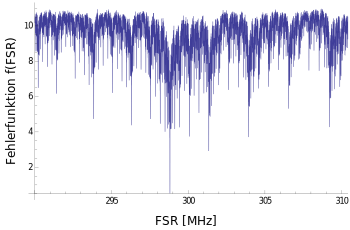
\includegraphics[width=(\textwidth-0.6cm)/2]{plt/nonius_FSR_messung_b}
		}\\
	 \subfloat[]{
		\label{subfig:nonius_FSR_messung_c}
		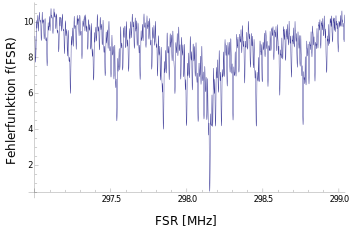
\includegraphics[width=(\textwidth-0.6cm)/2]{plt/nonius_FSR_messung_c}
		}
	\subfloat[]{
		\label{subfig:nonius_FSR_messung_d}
		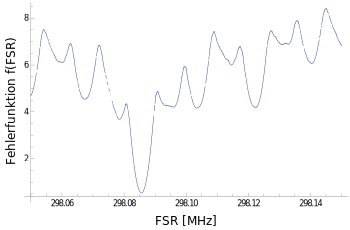
\includegraphics[width=(\textwidth-0.6cm)/2]{plt/nonius_FSR_messung_d}
		}
	}}
	\caption[FSR-Bestimmung]{Die Abbildung zeigt die Plots der Fehlerfunktionen.
	Von (a) nach (d) wurde der Ausschnitt des interessanten Minimums vergrößert. Die
	Stelle des Minimums ist der vermutliche FSR des FPIs.}
	\label{fig:nonius_FSR_messung}
\end{figure}

\subsection{Finesse}\label{subsec:finesse}
In diesem Abschnitt sollen kurz die Messungen der Finesse des FPIs
durchgesprochen werden. Im Gegensatz zum FSR ist die Finesse ein weniger
kritischer Parameter, sollte dennoch groß genug sein, damit die Spitze der
Transmissionsfringes genau mit der FOL-Technik präzise detektiert werden
kann. Wie in Abschn. \ref{subsec:fabry-perot-interferometer} erklärt, ist
die Finesse abhängig von der Wellenlänge des Laserlichts. Deshalb wurde für jeden
Wellenlängenbereich der in diesem System verwendenen Laser die Finesse
gemssen. Dazu wurde jeweils mithilfe eines Oszilloskops das Fringepattern der
steigenden Rampe aufgenommen und daran eine Airy-Funktion
\begin{equation}\label{eq:finesse_messung_01}
	U(t,\kappa,a,b,c) = b\cdot\frac{1}{1+\kappa \sin^2{(at)}}+c
\end{equation}
gefittet, wobei $U$ die verstärkte Spannung an der Photodiode, $t$ die Zeit,
$\kappa$ das Maß für die Finesse und $a$, $b$, $c$ Normierungsgrößen sind.
Abbildung \ref{fig:finesse_messung} zeigt die Plots inklusive Fits der
Fringepattern von \textit{DL-Pro} mit $772\,$nm (a), He:Ne-Laser mit $633\,$nm (b), und dem
blauen Diodenlaser mit $405\,$nm (c).

\begin{figure}[hp]
	\caption[Finesse des FPIs]{Die Abbildung zeigt die Plots des
 	Fringepattern für $772\,$nm (a), $633\,$nm (b) und $405\,$nm (c).}
	\label{fig:finesse_messung}
 	\centering
 	\footnotesize
 	\fbox{\parbox{\dimexpr \linewidth - 2\fboxrule - 2\fboxsep}{
 	\subfloat[]{
		\label{subfig:finesse_messung_a}
		% GNUPLOT: LaTeX picture with Postscript
\begingroup
  \makeatletter
  \providecommand\color[2][]{%
    \GenericError{(gnuplot) \space\space\space\@spaces}{%
      Package color not loaded in conjunction with
      terminal option `colourtext'%
    }{See the gnuplot documentation for explanation.%
    }{Either use 'blacktext' in gnuplot or load the package
      color.sty in LaTeX.}%
    \renewcommand\color[2][]{}%
  }%
  \providecommand\includegraphics[2][]{%
    \GenericError{(gnuplot) \space\space\space\@spaces}{%
      Package graphicx or graphics not loaded%
    }{See the gnuplot documentation for explanation.%
    }{The gnuplot epslatex terminal needs graphicx.sty or graphics.sty.}%
    \renewcommand\includegraphics[2][]{}%
  }%
  \providecommand\rotatebox[2]{#2}%
  \@ifundefined{ifGPcolor}{%
    \newif\ifGPcolor
    \GPcolortrue
  }{}%
  \@ifundefined{ifGPblacktext}{%
    \newif\ifGPblacktext
    \GPblacktexttrue
  }{}%
  % define a \g@addto@macro without @ in the name:
  \let\gplgaddtomacro\g@addto@macro
  % define empty templates for all commands taking text:
  \gdef\gplbacktext{}%
  \gdef\gplfronttext{}%
  \makeatother
  \ifGPblacktext
    % no textcolor at all
    \def\colorrgb#1{}%
    \def\colorgray#1{}%
  \else
    % gray or color?
    \ifGPcolor
      \def\colorrgb#1{\color[rgb]{#1}}%
      \def\colorgray#1{\color[gray]{#1}}%
      \expandafter\def\csname LTw\endcsname{\color{white}}%
      \expandafter\def\csname LTb\endcsname{\color{black}}%
      \expandafter\def\csname LTa\endcsname{\color{black}}%
      \expandafter\def\csname LT0\endcsname{\color[rgb]{1,0,0}}%
      \expandafter\def\csname LT1\endcsname{\color[rgb]{0,1,0}}%
      \expandafter\def\csname LT2\endcsname{\color[rgb]{0,0,1}}%
      \expandafter\def\csname LT3\endcsname{\color[rgb]{1,0,1}}%
      \expandafter\def\csname LT4\endcsname{\color[rgb]{0,1,1}}%
      \expandafter\def\csname LT5\endcsname{\color[rgb]{1,1,0}}%
      \expandafter\def\csname LT6\endcsname{\color[rgb]{0,0,0}}%
      \expandafter\def\csname LT7\endcsname{\color[rgb]{1,0.3,0}}%
      \expandafter\def\csname LT8\endcsname{\color[rgb]{0.5,0.5,0.5}}%
    \else
      % gray
      \def\colorrgb#1{\color{black}}%
      \def\colorgray#1{\color[gray]{#1}}%
      \expandafter\def\csname LTw\endcsname{\color{white}}%
      \expandafter\def\csname LTb\endcsname{\color{black}}%
      \expandafter\def\csname LTa\endcsname{\color{black}}%
      \expandafter\def\csname LT0\endcsname{\color{black}}%
      \expandafter\def\csname LT1\endcsname{\color{black}}%
      \expandafter\def\csname LT2\endcsname{\color{black}}%
      \expandafter\def\csname LT3\endcsname{\color{black}}%
      \expandafter\def\csname LT4\endcsname{\color{black}}%
      \expandafter\def\csname LT5\endcsname{\color{black}}%
      \expandafter\def\csname LT6\endcsname{\color{black}}%
      \expandafter\def\csname LT7\endcsname{\color{black}}%
      \expandafter\def\csname LT8\endcsname{\color{black}}%
    \fi
  \fi
  \setlength{\unitlength}{0.0500bp}%
  \begin{picture}(7936.00,3968.00)%
    \gplgaddtomacro\gplbacktext{%
      \csname LTb\endcsname%
      \put(980,640){\makebox(0,0)[r]{\strut{} 0}}%
      \put(980,1026){\makebox(0,0)[r]{\strut{} 0.01}}%
      \put(980,1412){\makebox(0,0)[r]{\strut{} 0.02}}%
      \put(980,1798){\makebox(0,0)[r]{\strut{} 0.03}}%
      \put(980,2184){\makebox(0,0)[r]{\strut{} 0.04}}%
      \put(980,2569){\makebox(0,0)[r]{\strut{} 0.05}}%
      \put(980,2955){\makebox(0,0)[r]{\strut{} 0.06}}%
      \put(980,3341){\makebox(0,0)[r]{\strut{} 0.07}}%
      \put(980,3727){\makebox(0,0)[r]{\strut{} 0.08}}%
      \put(1100,440){\makebox(0,0){\strut{}-6}}%
      \put(1909,440){\makebox(0,0){\strut{}-5}}%
      \put(2719,440){\makebox(0,0){\strut{}-4}}%
      \put(3528,440){\makebox(0,0){\strut{}-3}}%
      \put(4338,440){\makebox(0,0){\strut{}-2}}%
      \put(5147,440){\makebox(0,0){\strut{}-1}}%
      \put(5956,440){\makebox(0,0){\strut{} 0}}%
      \put(6766,440){\makebox(0,0){\strut{} 1}}%
      \put(7575,440){\makebox(0,0){\strut{} 2}}%
      \put(160,2183){\rotatebox{-270}{\makebox(0,0){\strut{}Amplitude U [V]}}}%
      \put(4337,140){\makebox(0,0){\strut{}Zeit t [ms]}}%
      \put(2719,2894){\makebox(0,0)[l]{\strut{}$\kappa = 992\pm14$}}%
      \put(2719,2677){\makebox(0,0)[l]{\strut{}$a = \unit{(562.020\pm0.044)}{\nicefrac{1}{s}}$}}%
      \put(2719,2461){\makebox(0,0)[l]{\strut{}$b = \unit{(0.05961\pm0.00028)}{V}$}}%
      \put(2719,2245){\makebox(0,0)[l]{\strut{}$c = \unit{(0.010994\pm0.000029)}{V}$}}%
    }%
    \gplgaddtomacro\gplfronttext{%
      \csname LTb\endcsname%
      \put(6672,3564){\makebox(0,0)[r]{\strut{}Fringepattern}}%
      \csname LTb\endcsname%
      \put(6672,3364){\makebox(0,0)[r]{\strut{}Fit}}%
    }%
    \gplbacktext
    \put(0,0){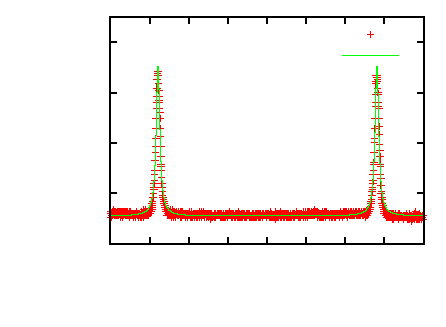
\includegraphics{finesse_messung_a}}%
    \gplfronttext
  \end{picture}%
\endgroup

		}\\
 	\subfloat[]{
		\label{subfig:finesse_messung_b}
		% GNUPLOT: LaTeX picture with Postscript
\begingroup
  \makeatletter
  \providecommand\color[2][]{%
    \GenericError{(gnuplot) \space\space\space\@spaces}{%
      Package color not loaded in conjunction with
      terminal option `colourtext'%
    }{See the gnuplot documentation for explanation.%
    }{Either use 'blacktext' in gnuplot or load the package
      color.sty in LaTeX.}%
    \renewcommand\color[2][]{}%
  }%
  \providecommand\includegraphics[2][]{%
    \GenericError{(gnuplot) \space\space\space\@spaces}{%
      Package graphicx or graphics not loaded%
    }{See the gnuplot documentation for explanation.%
    }{The gnuplot epslatex terminal needs graphicx.sty or graphics.sty.}%
    \renewcommand\includegraphics[2][]{}%
  }%
  \providecommand\rotatebox[2]{#2}%
  \@ifundefined{ifGPcolor}{%
    \newif\ifGPcolor
    \GPcolortrue
  }{}%
  \@ifundefined{ifGPblacktext}{%
    \newif\ifGPblacktext
    \GPblacktexttrue
  }{}%
  % define a \g@addto@macro without @ in the name:
  \let\gplgaddtomacro\g@addto@macro
  % define empty templates for all commands taking text:
  \gdef\gplbacktext{}%
  \gdef\gplfronttext{}%
  \makeatother
  \ifGPblacktext
    % no textcolor at all
    \def\colorrgb#1{}%
    \def\colorgray#1{}%
  \else
    % gray or color?
    \ifGPcolor
      \def\colorrgb#1{\color[rgb]{#1}}%
      \def\colorgray#1{\color[gray]{#1}}%
      \expandafter\def\csname LTw\endcsname{\color{white}}%
      \expandafter\def\csname LTb\endcsname{\color{black}}%
      \expandafter\def\csname LTa\endcsname{\color{black}}%
      \expandafter\def\csname LT0\endcsname{\color[rgb]{1,0,0}}%
      \expandafter\def\csname LT1\endcsname{\color[rgb]{0,1,0}}%
      \expandafter\def\csname LT2\endcsname{\color[rgb]{0,0,1}}%
      \expandafter\def\csname LT3\endcsname{\color[rgb]{1,0,1}}%
      \expandafter\def\csname LT4\endcsname{\color[rgb]{0,1,1}}%
      \expandafter\def\csname LT5\endcsname{\color[rgb]{1,1,0}}%
      \expandafter\def\csname LT6\endcsname{\color[rgb]{0,0,0}}%
      \expandafter\def\csname LT7\endcsname{\color[rgb]{1,0.3,0}}%
      \expandafter\def\csname LT8\endcsname{\color[rgb]{0.5,0.5,0.5}}%
    \else
      % gray
      \def\colorrgb#1{\color{black}}%
      \def\colorgray#1{\color[gray]{#1}}%
      \expandafter\def\csname LTw\endcsname{\color{white}}%
      \expandafter\def\csname LTb\endcsname{\color{black}}%
      \expandafter\def\csname LTa\endcsname{\color{black}}%
      \expandafter\def\csname LT0\endcsname{\color{black}}%
      \expandafter\def\csname LT1\endcsname{\color{black}}%
      \expandafter\def\csname LT2\endcsname{\color{black}}%
      \expandafter\def\csname LT3\endcsname{\color{black}}%
      \expandafter\def\csname LT4\endcsname{\color{black}}%
      \expandafter\def\csname LT5\endcsname{\color{black}}%
      \expandafter\def\csname LT6\endcsname{\color{black}}%
      \expandafter\def\csname LT7\endcsname{\color{black}}%
      \expandafter\def\csname LT8\endcsname{\color{black}}%
    \fi
  \fi
  \setlength{\unitlength}{0.0500bp}%
  \begin{picture}(3968.00,2834.00)%
    \gplgaddtomacro\gplbacktext{%
      \csname LTb\endcsname%
      \put(660,896){\makebox(0,0)[r]{\strut{} 0}}%
      \put(660,1407){\makebox(0,0)[r]{\strut{} 0.2}}%
      \put(660,1918){\makebox(0,0)[r]{\strut{} 0.4}}%
      \put(660,2430){\makebox(0,0)[r]{\strut{} 0.6}}%
      \put(780,440){\makebox(0,0){\strut{}-2}}%
      \put(1227,440){\makebox(0,0){\strut{}-1}}%
      \put(1673,440){\makebox(0,0){\strut{} 0}}%
      \put(2120,440){\makebox(0,0){\strut{} 1}}%
      \put(2567,440){\makebox(0,0){\strut{} 2}}%
      \put(3014,440){\makebox(0,0){\strut{} 3}}%
      \put(3460,440){\makebox(0,0){\strut{} 4}}%
      \put(3907,440){\makebox(0,0){\strut{} 5}}%
      \put(200,1726){\rotatebox{-270}{\makebox(0,0){\strut{}Amplitude U [V]}}}%
      \put(2343,140){\makebox(0,0){\strut{}Zeit t [ms]}}%
      \put(1562,1944){\makebox(0,0)[l]{\strut{}\tiny$\kappa = 522.6\pm6.9$}}%
      \put(1562,1727){\makebox(0,0)[l]{\strut{}\tiny$a = (686.405\pm0.068)\,$s$^{-1}$}}%
      \put(1562,1509){\makebox(0,0)[l]{\strut{}\tiny$b = (0.5879\pm0.0026)\,$V}}%
      \put(1562,1292){\makebox(0,0)[l]{\strut{}\tiny$c = (-0.02542\pm0.00035)\,$V}}%
    }%
    \gplgaddtomacro\gplfronttext{%
      \csname LTb\endcsname%
      \put(3004,2650){\makebox(0,0)[r]{\strut{}Fringepattern}}%
      \csname LTb\endcsname%
      \put(3004,2450){\makebox(0,0)[r]{\strut{}Fit}}%
    }%
    \gplbacktext
    \put(0,0){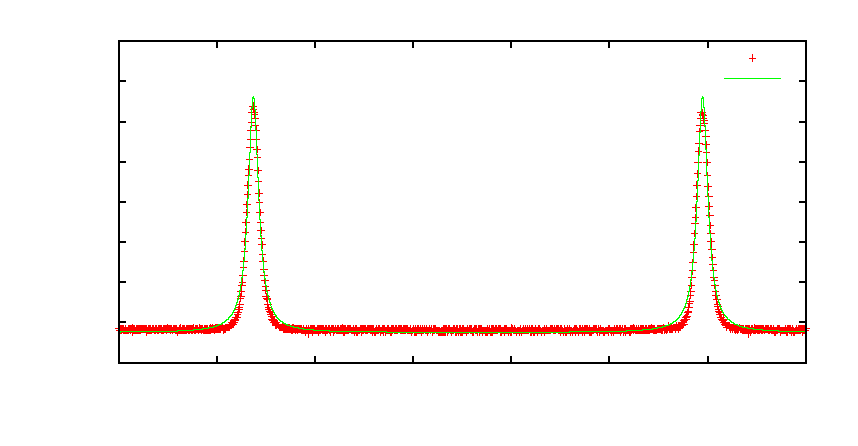
\includegraphics{finesse_messung_b}}%
    \gplfronttext
  \end{picture}%
\endgroup

		}\\
	 \subfloat[]{
		\label{subfig:finesse_messung_c}
		% GNUPLOT: LaTeX picture with Postscript
\begingroup
  \makeatletter
  \providecommand\color[2][]{%
    \GenericError{(gnuplot) \space\space\space\@spaces}{%
      Package color not loaded in conjunction with
      terminal option `colourtext'%
    }{See the gnuplot documentation for explanation.%
    }{Either use 'blacktext' in gnuplot or load the package
      color.sty in LaTeX.}%
    \renewcommand\color[2][]{}%
  }%
  \providecommand\includegraphics[2][]{%
    \GenericError{(gnuplot) \space\space\space\@spaces}{%
      Package graphicx or graphics not loaded%
    }{See the gnuplot documentation for explanation.%
    }{The gnuplot epslatex terminal needs graphicx.sty or graphics.sty.}%
    \renewcommand\includegraphics[2][]{}%
  }%
  \providecommand\rotatebox[2]{#2}%
  \@ifundefined{ifGPcolor}{%
    \newif\ifGPcolor
    \GPcolortrue
  }{}%
  \@ifundefined{ifGPblacktext}{%
    \newif\ifGPblacktext
    \GPblacktexttrue
  }{}%
  % define a \g@addto@macro without @ in the name:
  \let\gplgaddtomacro\g@addto@macro
  % define empty templates for all commands taking text:
  \gdef\gplbacktext{}%
  \gdef\gplfronttext{}%
  \makeatother
  \ifGPblacktext
    % no textcolor at all
    \def\colorrgb#1{}%
    \def\colorgray#1{}%
  \else
    % gray or color?
    \ifGPcolor
      \def\colorrgb#1{\color[rgb]{#1}}%
      \def\colorgray#1{\color[gray]{#1}}%
      \expandafter\def\csname LTw\endcsname{\color{white}}%
      \expandafter\def\csname LTb\endcsname{\color{black}}%
      \expandafter\def\csname LTa\endcsname{\color{black}}%
      \expandafter\def\csname LT0\endcsname{\color[rgb]{1,0,0}}%
      \expandafter\def\csname LT1\endcsname{\color[rgb]{0,1,0}}%
      \expandafter\def\csname LT2\endcsname{\color[rgb]{0,0,1}}%
      \expandafter\def\csname LT3\endcsname{\color[rgb]{1,0,1}}%
      \expandafter\def\csname LT4\endcsname{\color[rgb]{0,1,1}}%
      \expandafter\def\csname LT5\endcsname{\color[rgb]{1,1,0}}%
      \expandafter\def\csname LT6\endcsname{\color[rgb]{0,0,0}}%
      \expandafter\def\csname LT7\endcsname{\color[rgb]{1,0.3,0}}%
      \expandafter\def\csname LT8\endcsname{\color[rgb]{0.5,0.5,0.5}}%
    \else
      % gray
      \def\colorrgb#1{\color{black}}%
      \def\colorgray#1{\color[gray]{#1}}%
      \expandafter\def\csname LTw\endcsname{\color{white}}%
      \expandafter\def\csname LTb\endcsname{\color{black}}%
      \expandafter\def\csname LTa\endcsname{\color{black}}%
      \expandafter\def\csname LT0\endcsname{\color{black}}%
      \expandafter\def\csname LT1\endcsname{\color{black}}%
      \expandafter\def\csname LT2\endcsname{\color{black}}%
      \expandafter\def\csname LT3\endcsname{\color{black}}%
      \expandafter\def\csname LT4\endcsname{\color{black}}%
      \expandafter\def\csname LT5\endcsname{\color{black}}%
      \expandafter\def\csname LT6\endcsname{\color{black}}%
      \expandafter\def\csname LT7\endcsname{\color{black}}%
      \expandafter\def\csname LT8\endcsname{\color{black}}%
    \fi
  \fi
  \setlength{\unitlength}{0.0500bp}%
  \begin{picture}(3968.00,2834.00)%
    \gplgaddtomacro\gplbacktext{%
      \csname LTb\endcsname%
      \put(500,640){\makebox(0,0)[r]{\strut{} 1}}%
      \put(500,1112){\makebox(0,0)[r]{\strut{} 2}}%
      \put(500,1585){\makebox(0,0)[r]{\strut{} 3}}%
      \put(500,2057){\makebox(0,0)[r]{\strut{} 4}}%
      \put(500,2530){\makebox(0,0)[r]{\strut{} 5}}%
      \put(894,440){\makebox(0,0){\strut{}-2}}%
      \put(1442,440){\makebox(0,0){\strut{}-1}}%
      \put(1990,440){\makebox(0,0){\strut{} 0}}%
      \put(2537,440){\makebox(0,0){\strut{} 1}}%
      \put(3085,440){\makebox(0,0){\strut{} 2}}%
      \put(3633,440){\makebox(0,0){\strut{} 3}}%
      \put(160,1726){\rotatebox{-270}{\makebox(0,0){\strut{}Amplitude U [V]}}}%
      \put(2263,140){\makebox(0,0){\strut{}Zeit t [ms]}}%
      \put(1442,1401){\makebox(0,0)[l]{\strut{}\tiny$\kappa = 1.515\pm0.026$}}%
      \put(1442,1227){\makebox(0,0)[l]{\strut{}\tiny$a = (1065.75\pm0.51)\,$s$^{-1}$}}%
      \put(1442,1053){\makebox(0,0)[l]{\strut{}\tiny$b = (2.917\pm0.020)\,$V}}%
      \put(1442,879){\makebox(0,0)[l]{\strut{}\tiny$c = (1.690\pm0.022)\,$V}}%
    }%
    \gplgaddtomacro\gplfronttext{%
      \csname LTb\endcsname%
      \put(3004,2650){\makebox(0,0)[r]{\strut{}Fringepattern}}%
      \csname LTb\endcsname%
      \put(3004,2450){\makebox(0,0)[r]{\strut{}Fit}}%
    }%
    \gplbacktext
    \put(0,0){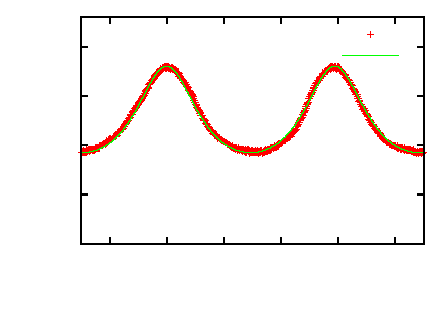
\includegraphics{finesse_messung_c}}%
    \gplfronttext
  \end{picture}%
\endgroup

		}
	}}
\end{figure}
Aus den Fits lassen sich die jeweiligen Reflektivitäten der Spiegel für die
Wellenlängen über
\begin{equation}\label{eq:finesse_messung_02}
	\begin{split}
		\kappa&=\frac{4R}{(1-R)^2}\\
		&\Leftrightarrow\\
		R&=\frac{2+\kappa-2\sqrt{1+\kappa}}{\kappa}
	\end{split}	
\end{equation}
berechnen. Tabelle \ref{tab:finesse} führt alle Reflektivitäten und Finessen
(nach \ref{eq:FPI_finesse}) auf. Wie schon in Abschn. \ref{sec:lasersystem}
erwähnt, hat das FPI im blauen Bereich eine sehr schlechte Finesse, mit der
allerdings immernoch gearbeitet werden kann. Im infraroten Bereich hat das FPI
offensichtlich die höchste Finesse.
\begin{table}[h]
	%Summe der Breiten muss 0.91 mal \textwidth sein.
	\begin{tabular}{ccc}
		\toprule
		\multicolumn{1}{C{0.30\textwidth}}{Wellenlänge [nm]} &
		\multicolumn{1}{C{0.31\textwidth}}{Spiegelreflektivität} &
		\multicolumn{1}{C{0.30\textwidth}}{Finesse}\\
		\midrule[1px]
		\hline
		%%%%%%%%%%%%%%%%%%%%%%%%%%%%%%%%%%%%%%%%%%%%%%%%%%%%%%%%%%%%%%%%%%%%%%
%%                                                                  %%
%%  This is a LaTeX2e table fragment exported from Gnumeric.        %%
%%                                                                  %%
%%%%%%%%%%%%%%%%%%%%%%%%%%%%%%%%%%%%%%%%%%%%%%%%%%%%%%%%%%%%%%%%%%%%%%
%Wellenlänge [nm]	&Spiegelreflektivität	&Finesse\\
772	&0,93848(42)	&49,47(35)\\
633	&0,91626(53)	&35,90(24)\\
405	&0,2266(25)	&1,656(21)\\
		\bottomrule[1px]
	\end{tabular}
	\caption[FPI Finesse]{Aufgelistet sind die Messwerte für die Reflektivität der
	Spiegel und die Finesse des FPIs in Abhängigkeit von der Wellenlänge.}
	\label{tab:finesse}
\end{table}

\section{Stabilität der Laser}\label{sec:stabilitaet_der_laser}
Um die Lang- und Kurzzeitstabilität der Laser zu untersuchen wurden zwei
verschiedene Methoden angewandt. Zum einen wurde sowohl vom alten als auch vom
neuen Lasersystem das Frequenzverhalten mithilfe der neu entwickelte Software
aufgezeichnet. Zum anderen haben Schwebungsfrequenzmessungen zweier Laser mit
der nahezu gleichen Frequenz Relativfrequenzdaten beider Laser geliefert. Die
Ergebnisse dieser beiden Methoden sollen in diesem Abschnitt vorgestellt werden.
Dabei wurde das alte System ausschließlich mit der alten und das neue
ausschließlich mit der im Ramen dieser Arbeit entwickelten Regelung
stabilsiliert.

\subsection{Stabilitätsmessung mit neuer
Software}\label{sec:stabilitaetsmessungen_software} Das Frequenzverhalten
aller drei Laser des neuen Systems wurde mit der neu entwickelten Software über zwei Stunden hinweg analysiert, wobei die
Laser jeweils freilaufend, \textit{iScan}-stabilsiert und
\textit{iScan}+FOL-stabilisiert gemessen wurden. Weiterhin wurde das
Frequenzverhalten des Lasers für den zweiten Anregungsschritt aus dem alten Lasersystem mit der neuen Software aufgezeichnet,
während dieser mit der alten FOL-Technik stabilisiert wurde.\par
\begin{figure}[h]
 	\centering
 	\footnotesize
	% GNUPLOT: LaTeX picture with Postscript
\begingroup
  \makeatletter
  \providecommand\color[2][]{%
    \GenericError{(gnuplot) \space\space\space\@spaces}{%
      Package color not loaded in conjunction with
      terminal option `colourtext'%
    }{See the gnuplot documentation for explanation.%
    }{Either use 'blacktext' in gnuplot or load the package
      color.sty in LaTeX.}%
    \renewcommand\color[2][]{}%
  }%
  \providecommand\includegraphics[2][]{%
    \GenericError{(gnuplot) \space\space\space\@spaces}{%
      Package graphicx or graphics not loaded%
    }{See the gnuplot documentation for explanation.%
    }{The gnuplot epslatex terminal needs graphicx.sty or graphics.sty.}%
    \renewcommand\includegraphics[2][]{}%
  }%
  \providecommand\rotatebox[2]{#2}%
  \@ifundefined{ifGPcolor}{%
    \newif\ifGPcolor
    \GPcolortrue
  }{}%
  \@ifundefined{ifGPblacktext}{%
    \newif\ifGPblacktext
    \GPblacktexttrue
  }{}%
  % define a \g@addto@macro without @ in the name:
  \let\gplgaddtomacro\g@addto@macro
  % define empty templates for all commands taking text:
  \gdef\gplbacktext{}%
  \gdef\gplfronttext{}%
  \makeatother
  \ifGPblacktext
    % no textcolor at all
    \def\colorrgb#1{}%
    \def\colorgray#1{}%
  \else
    % gray or color?
    \ifGPcolor
      \def\colorrgb#1{\color[rgb]{#1}}%
      \def\colorgray#1{\color[gray]{#1}}%
      \expandafter\def\csname LTw\endcsname{\color{white}}%
      \expandafter\def\csname LTb\endcsname{\color{black}}%
      \expandafter\def\csname LTa\endcsname{\color{black}}%
      \expandafter\def\csname LT0\endcsname{\color[rgb]{1,0,0}}%
      \expandafter\def\csname LT1\endcsname{\color[rgb]{0,1,0}}%
      \expandafter\def\csname LT2\endcsname{\color[rgb]{0,0,1}}%
      \expandafter\def\csname LT3\endcsname{\color[rgb]{1,0,1}}%
      \expandafter\def\csname LT4\endcsname{\color[rgb]{0,1,1}}%
      \expandafter\def\csname LT5\endcsname{\color[rgb]{1,1,0}}%
      \expandafter\def\csname LT6\endcsname{\color[rgb]{0,0,0}}%
      \expandafter\def\csname LT7\endcsname{\color[rgb]{1,0.3,0}}%
      \expandafter\def\csname LT8\endcsname{\color[rgb]{0.5,0.5,0.5}}%
    \else
      % gray
      \def\colorrgb#1{\color{black}}%
      \def\colorgray#1{\color[gray]{#1}}%
      \expandafter\def\csname LTw\endcsname{\color{white}}%
      \expandafter\def\csname LTb\endcsname{\color{black}}%
      \expandafter\def\csname LTa\endcsname{\color{black}}%
      \expandafter\def\csname LT0\endcsname{\color{black}}%
      \expandafter\def\csname LT1\endcsname{\color{black}}%
      \expandafter\def\csname LT2\endcsname{\color{black}}%
      \expandafter\def\csname LT3\endcsname{\color{black}}%
      \expandafter\def\csname LT4\endcsname{\color{black}}%
      \expandafter\def\csname LT5\endcsname{\color{black}}%
      \expandafter\def\csname LT6\endcsname{\color{black}}%
      \expandafter\def\csname LT7\endcsname{\color{black}}%
      \expandafter\def\csname LT8\endcsname{\color{black}}%
    \fi
  \fi
  \setlength{\unitlength}{0.0500bp}%
  \begin{picture}(8502.00,6802.00)%
    \gplgaddtomacro\gplbacktext{%
      \csname LTb\endcsname%
      \put(1080,3401){\makebox(0,0)[r]{\strut{}-60}}%
      \put(1080,3796){\makebox(0,0)[r]{\strut{}-50}}%
      \put(1080,4191){\makebox(0,0)[r]{\strut{}-40}}%
      \put(1080,4586){\makebox(0,0)[r]{\strut{}-30}}%
      \put(1080,4981){\makebox(0,0)[r]{\strut{}-20}}%
      \put(1080,5376){\makebox(0,0)[r]{\strut{}-10}}%
      \put(1080,5771){\makebox(0,0)[r]{\strut{} 0}}%
      \put(1080,6166){\makebox(0,0)[r]{\strut{} 10}}%
      \put(1080,6561){\makebox(0,0)[r]{\strut{} 20}}%
      \put(1200,3201){\makebox(0,0){\strut{}}}%
      \put(2357,3201){\makebox(0,0){\strut{}}}%
      \put(3514,3201){\makebox(0,0){\strut{}}}%
      \put(4671,3201){\makebox(0,0){\strut{}}}%
      \put(5827,3201){\makebox(0,0){\strut{}}}%
      \put(6984,3201){\makebox(0,0){\strut{}}}%
      \put(8141,3201){\makebox(0,0){\strut{}}}%
      \put(500,4981){\rotatebox{-270}{\makebox(0,0){\strut{}relative Frequenz [MHz]}}}%
    }%
    \gplgaddtomacro\gplfronttext{%
      \csname LTb\endcsname%
      \put(5040,3964){\makebox(0,0)[r]{\strut{}freilaufend}}%
      \csname LTb\endcsname%
      \put(5040,3764){\makebox(0,0)[r]{\strut{}\textit{iScan}-stabilisiert}}%
      \csname LTb\endcsname%
      \put(5040,3564){\makebox(0,0)[r]{\strut{}\textit{iScan}+FOL-stabilisiert}}%
    }%
    \gplgaddtomacro\gplbacktext{%
      \csname LTb\endcsname%
      \put(1080,2585){\makebox(0,0)[r]{\strut{} 0.5}}%
      \put(1080,2791){\makebox(0,0)[r]{\strut{} 1}}%
      \put(1080,2996){\makebox(0,0)[r]{\strut{} 1.5}}%
      \put(1200,2180){\makebox(0,0){\strut{}}}%
      \put(2357,2180){\makebox(0,0){\strut{}}}%
      \put(3514,2180){\makebox(0,0){\strut{}}}%
      \put(4671,2180){\makebox(0,0){\strut{}}}%
      \put(5827,2180){\makebox(0,0){\strut{}}}%
      \put(6984,2180){\makebox(0,0){\strut{}}}%
      \put(8141,2180){\makebox(0,0){\strut{}}}%
    }%
    \gplgaddtomacro\gplfronttext{%
    }%
    \gplgaddtomacro\gplbacktext{%
      \csname LTb\endcsname%
      \put(1080,1615){\makebox(0,0)[r]{\strut{} 0.5}}%
      \put(1080,1870){\makebox(0,0)[r]{\strut{} 1}}%
      \put(1080,2125){\makebox(0,0)[r]{\strut{} 1.5}}%
      \put(1200,1160){\makebox(0,0){\strut{}}}%
      \put(2357,1160){\makebox(0,0){\strut{}}}%
      \put(3514,1160){\makebox(0,0){\strut{}}}%
      \put(4671,1160){\makebox(0,0){\strut{}}}%
      \put(5827,1160){\makebox(0,0){\strut{}}}%
      \put(6984,1160){\makebox(0,0){\strut{}}}%
      \put(8141,1160){\makebox(0,0){\strut{}}}%
      \put(500,1870){\rotatebox{-270}{\makebox(0,0){\strut{}Jitter [MHz]}}}%
    }%
    \gplgaddtomacro\gplfronttext{%
    }%
    \gplgaddtomacro\gplbacktext{%
      \csname LTb\endcsname%
      \put(1080,790){\makebox(0,0)[r]{\strut{} 0.5}}%
      \put(1080,980){\makebox(0,0)[r]{\strut{} 1}}%
      \put(1080,1170){\makebox(0,0)[r]{\strut{} 1.5}}%
      \put(1200,400){\makebox(0,0){\strut{}0}}%
      \put(2357,400){\makebox(0,0){\strut{}20}}%
      \put(3514,400){\makebox(0,0){\strut{}40}}%
      \put(4671,400){\makebox(0,0){\strut{}60}}%
      \put(5827,400){\makebox(0,0){\strut{}80}}%
      \put(6984,400){\makebox(0,0){\strut{}100}}%
      \put(8141,400){\makebox(0,0){\strut{}120}}%
      \put(4670,100){\makebox(0,0){\strut{}Zeit [min]}}%
    }%
    \gplgaddtomacro\gplfronttext{%
    }%
    \gplbacktext
    \put(0,0){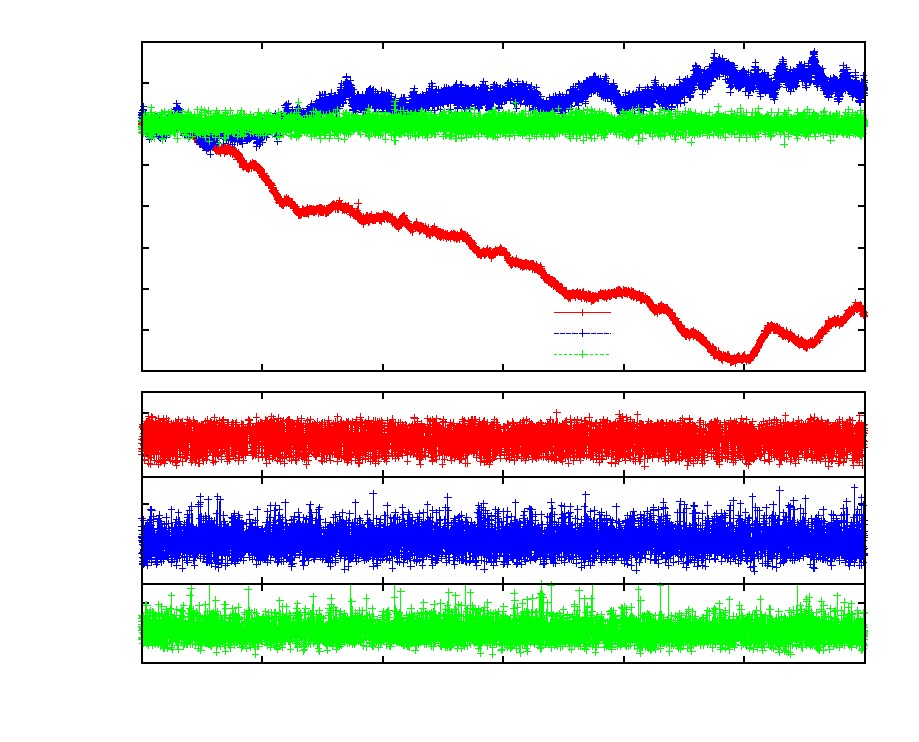
\includegraphics{laserstabilitaet_b_alles}}%
    \gplfronttext
  \end{picture}%
\endgroup

	\caption[Laserfrequenzverhalten \textit{DL-Pro}]{Die Abbildung zeigt das
	Laserfrequenzverhalten des \textit{DL-Pro} im freilaufenden (rot),
	\textit{iScan}-stabiliserten (blau) und \textit{iScan}+FOL-stabiliserten Modus
	(grün).
	Unten ist jeweils entsprechend farblich kodiert der Jitter aufgetragen.
	Separate, hochaufgelöstere Plots für alle Laser finden sich in Anh.
	\ref{anh:sec:laserstabilitaet}.}
	\label{fig:laserstabilitaet_b_alles}
\end{figure}
Abbildung \ref{fig:laserstabilitaet_b_alles} zeigt den relativen
Frequenzverlauf des \textit{DL-Pro} im freilaufenden (rot),
\textit{iScan}-stabiliserten (blau) und \textit{iScan}+FOL-stabiliserten Modus
(grün). Die Plots für die anderen beiden Laser befinden sich in Anh.
\ref{anh:sec:laserstabilitaet}. Sind die Laser nicht aktiv stabilisiert, driften
sie deutlich in der Frequenz. Der \textit{DL-Pro} driftet in zwei Stunden bis zu $60\,$MHz, wohingehen der
\textit{TA-Pro} nur einen maximalen Drift von $20\,$MHz vorweist. Dieser
Unterschied ist allerdings keine Systematik, da auch beim \textit{TA-Pro} schon
größere Drifts beobachtet wurden. Sehr viel größere Frequenzfluktuationen (bis $700\,$MHz)
weist der blaue Laser auf, was auf die wesentlich instabilere Mechanik
zurückzuführen ist. Größtenteils sind die Drift vermutlich mit der Temperatur
korreliert, was hier allerdings nicht nachgeprüft wurde. Eine weitere Ursache
ist der Piezoaktuator des Gitters, der nach Ändern der Spannung noch lange in
die gleiche Richtung nachdriftet. Der Jitter der Laser (Standardabweichung der
Frequenz über die durch den \textit{Arduino} gemittelten Werte) liegt für die
beiden \textit{Toptica}-Lasern bei maximal $1,5\,$MHz. Für den blauen Laser
liegt dieser bei etwa $5\,$MHz.\par
Wie erwartet reduziert sich der Drift bei \textit{iScan}-Stabilisierung,
verschwindet aber leider nicht völlig (immernoch ca. $20\,$MHz). Für den \textit{TA-Pro} ist die
\textit{iScan}-Stabilisierung kein besonderer Mehrgewinn, was allerdings wie
schon erwähnt nur speziell auf diese Messung zutreffend ist. Der blaue Laser
erfährt einen dramatischen Zugewinn an Stabilität mit einer Reduzierung des
Drifts auf ca. $100\,$MHz. Es zeigt sich, dass die \textit{iScans} zwar
eine hinreichend gute Stabilität in kurzen Zeitintervallen gewährleisten, jedoch
auf größeren Zeitskalen systematischen Schwankungen ausgeliefert sind. Die
wahrscheinlichste Ursache ist die sensible räumliche Abhängigkeit der
Einkopplung in die \textit{iScan heads}, was sich durch eine alternative
Faserkopplung überprüfen ließe. Eine weitere Ursache könnte trotz
Temperaturkontrolle die fehlende aktive Stabilisierung der internen \textit{iScan}-Optik sein. Der
Jitter ändert sich im Vergleich zum freilaufenden Fall nicht merklich,
weist aber ab und zu kleinere Überhöhungen auf, die mit der Regelung der
\textit{iScans} und/oder des FOL zu erklären sind.\par
%TODO: evtl. periodische Schwingung des Jitters erwähnen
Um die Drifts völlig zu eliminieren, muss das FOL hinzugeschaltet werden. Wie
Abb. \ref{fig:laserstabilitaet_b_alles} zeigt, reduziert sich
dank des FOL der Drift auf nahezu $0\,$MHz. Die Fluktuationen um die
Soll-Relativfrequenz (hier $0\,$MHz) ergibt sich nur noch aus dem Jitter der
Laser und der Regelung des FOL zu maximal $\pm12\,$MHz für den blauen und
$\pm4\,$MHz für die beiden roten Laser. Dieses Frequenzrauschen lässt sich ggf.
noch durch Variieren der Ober- und Untergrenzen für das FOL verkleinern, kann aber bei zu eng
gewählten Grenzen zu Überreglung und somit zu größeren Fluktuationen führen.\par
\begin{figure}[h]
 	\centering
 	\footnotesize
	\input{plt/laserstabilitaet_alt_alles}
	\caption[Laserfrequenzverhalten altes System]{Die Abbildung zeigt das
	Frequenzverhalten des Lasers für den zweiten Anregungsschritts im alten System
	im freilaufenden (rot) und FOL-stabiliserten Modus (grün).
	Unten ist jeweils in des entsprechenden Farben der Jitter aufgetragen.
	Separate, hochaufgelöstere Plots hierfür finden sich in Anh.
	\ref{anh:sec:laserstabilitaet}.}
	\label{fig:laserstabilitaet_alt_alles}
\end{figure}
Abbildung \ref{fig:laserstabilitaet_alt_alles} zeigt die Plots für den
roten Laser des zweiten Anregungsschritts im alten System, dessen Daten auch über zwei Stunden aber mit einer
höreren Rate\footnote{Die Daten wurden zu einem Zeitpunkt aufgenommen, an dem die Software schon in einem performanteren
Stadium war und mit einer höheren Rate Laserdaten verarbeiten konnte.}
aufgenommen wurden (rot: freilaufend;
grün: FOL-stabilisiert). Seperate, hochaufgelöstere Plots finden sich im Anh.
\ref{anh:sec:laserstabilitaet}. Im freilaufenden Modus driftet der Laser bis
zu $300\,$MHz in zwei Stunden. Der Jitter liegt im Mittel bei etwa $5\,$MHz und
ist max $15\,$MHz, wurde aber auf der Grundlage weniger Rampenzyklen berechnet
und muss deshalb in der Größenordnung von $100\,$ms angesiedelt werden. Es zeigt sich, dass die
Frequenzfluktuation darüber hinaus aber in der Größenordnung von mehreren
Sekunden gut $100\,$MHz beträgt, was normalerweise für die Laser dieser Bauart
nicht üblich ist. Ein möglicher Grund können Schwebungen von Vibrationen sein,
die beispielsweise durch die Vorpumpe der Vakuumaparatur ausgelöst werden. Im
stabilisierten Modus zeigt der Laser ein vergleichbares Verhalten mit
dem blauen Laser aus dem neuen System, was aufgrund der gleichen Bauart nicht
verwunderlich ist. Der Jitter fluktuiert hier scheinbar mehr als beim blauen
Laser. Dies liegt aber daran, dass hier seitens des \textit{Arduinos} über
wesentlich weniger Werte gemittelt wurde. Auch verschindet erfreulicherweise der
makroskopische Jitter.\par
In der Effizienz der aktiven Stabilisierung unterscheiden sich die beiden
Lasersysteme also nicht merklich. Der einzige offensichtliche Vorteil des neuen
Systems liegt in der Bauweise der \textit{Toptica}-Laser, die die
Grundstabilität enorm steigert. Fluktuationen wie im Falle des Lasers aus dem
alten System werden somit von Grund auf unterdrückt.

\subsection{Stabilitätsmessung über
Schwebungsfrequenzen}\label{subsec:beatfrequenzmessung}
\begin{figure}[hp]
 	\centering
 	\footnotesize
 	\fbox{\parbox{\dimexpr \linewidth - 2\fboxrule - 2\fboxsep}{
 	\subfloat[]{
		\label{subfig:beatfrequenzmessung_aufbau_schematisch}
		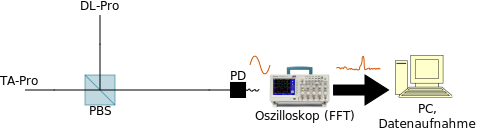
\includegraphics[width=\textwidth-2cm]{gfx/beatfrequenzmessung_aufbau_schematisch}
		}\\
 	\subfloat[]{
		\label{subfig:beatfrequenzen_signal}
		\input{plt/beatfrequenzen_signal}
		}\\
	 \subfloat[]{
		\label{subfig:beatfrequenzen_fft}
		\input{plt/beatfrequenzen_fft}
		}
	}}
	\caption[Beatfrequenzmessung]{Die Zeichnung (a) zeigt den Aufbau der
	Schwebungsfrequenzmessung. In (b) ist das Schwebungssignal über einen
	Ausschnitt von $500\,$ns dargestellt. (c) ist die Fouriertransformierte dieses
	Signals. Weitere Erklärungen finden sich im Text. ((b) und (c) sind nur
	exemplarische Darstellungen und sind nicht miteinander korreliert.)}
	\label{fig:beatfrequenzmessung}
\end{figure}
Um die Aussagekraft der Messungen im vorherigen Abschnitt durch eine wesentlich
direktere Methode zur Relativfrequenzanalyse zu überprüfen, eignet sich hervorragend die
Messung von Schwebungsfrequenzen der beiden roten Laser. Dazu wurden wie in Abb.
\ref{fig:beatfrequenzmessung}\subref{subfig:beatfrequenzmessung_aufbau_schematisch}
schematisch dargestellt jeweils ein Teilstrahl der beiden Laser mit einen Polarisationsstrahlteiler
überlagert und auf eine Photodiode geschickt. Bringt man nun die Frequenzen
beider Laser auf nahe beieinander liegende Frequenzen (wenige MHz
Unterschied), entsteht durch Interferenz beider
elektromagnetischen Felder ein Schwebungssignal mit der Differenzfrequenz der
beiden Laserfrequenzen (siehe Abb.
\ref{fig:beatfrequenzmessung}\subref{subfig:beatfrequenzen_signal}), welches über den Strom der Photodiode an einem Oszilloskop über die \textit{Fast-Fourier-Transformation} (FFT)
spektral analysiert werden kann. Pro Messung wurden so über einige Minuten
mehrere $1000$ Frequenzspektren aufgenommen und mithilfe eines selbst
geschriebenen \textit{Python}-Skripts und \textit{GnuPlot} an ein Gaußprofil
angefittet (siehe exemplarisch
\ref{fig:beatfrequenzmessung}\subref{subfig:beatfrequenzen_fft}).
Sowohl für das neue als auch für das alte System wurden bei stabilisierten
Lasern Schwebungssignale analysiert. Unstabilisiert ist es praktisch nicht
möglich einen Frequenzverlauf aufzuzeichnen, da die Laser schnell in zu
großen Differenzfreuqenzen driften. Zum einen bricht das Schwebungssignal
bei großen Schwebungsfrequnzen ($>30\,$MHz) fast völlig ein und kann nicht mehr
analysiert werden. Zum anderen treten Zweideutigkeiten auf, wenn die
Differenzfrequenz ihr Vorzeichen wechselt, was durchaus eintreten kann, wenn die
Laser zu Beginn in der Frequenz nur wenige MHz auseinander liegen.\par
Beim neuen System wurden die Schwebungsfrequenzen sowohl nur mit
\textit{iScan}-Stabilisierung als auch mit der Kombination von \textit{iScan}
und FOL aufgenommen.
\begin{figure}[hp]
 	\centering
 	\footnotesize
 	\fbox{\parbox{\dimexpr \linewidth - 2\fboxrule - 2\fboxsep}{
 	\subfloat[]{
		\label{subfig:beatfrequenzen_neu_iScan_drift}
		\input{plt/beatfrequenzen_neu_iScan_drift}
		}\\
 	\subfloat[]{
		\label{subfig:beatfrequenzen_neu_iScan_histogramm}
		\input{plt/beatfrequenzen_neu_iScan_histogramm}
		}
	}}
	\caption[Beatfrequenzen - neues System mit \textit{iScan}]{In (a) ist der
	Frequenzverlauf des Schwebungssignals der beiden roten
	\textit{iScan}-stabilisierten Laser des neuen Systems über eine Zeit von
	$65\,$min zu sehen.
	(b) zeigt die Frequenzverteilung in den ersten $9\,$min der Messung (grauer Bereich in (a)).}
	\label{fig:beatfrequenzen_neu_iScan}
\end{figure}
Abbildung
\ref{fig:beatfrequenzen_neu_iScan}\subref{subfig:beatfrequenzen_neu_iScan_drift} zeigt den Frequenzverlauf des Schwebungssignals über einen Zeitraum von $65\,$min mit
\textit{iScan}-Regelung. Die Fehlerbalken resultieren aus den
Standardabweichungen der einzelnen Gauß-Fits. Es ist ein leichter Drift von
maximal $10\,$MHz zu erkennen, welcher in der Größenordnung mit den
einzelnen Drifts der beiden Laser bei den Messungen des vorherigen Abschnitts
übereinstimmt. Dort sind die beide Laser jeweils in der gleichen Zeit ca.
$10\,$MHz gedriftet. Zu beachten ist, dass synchrone Drifts beider Laser (evtl.
Temperaturdrifts) keine Auswirkungen auf Schwebungsfrequenzdrifts haben. Um eine
quantitativ gesicherte Aussage über den Vergleich beider Messungen machen zu
können, wären viele Einzelmessungen (Statistik) nötig, was einen erheblichen
Mehraufwand bedeuten würde. Die Messung der Schwebungsfrequenzen liefert also
bezüglich des Drifts qualitativ die gleiche Aussage wie die Messungen mit der
neuen Software. Weiterhin kann eine quantitative Aussage über die Fluktuation
der Laserfrequenzen in kleinen Zeitskalen bei eingeschalteter
\textit{iScan}-Stabilisierung getroffen werden. Dazu wurde für die ersten
$9\,$min der Messung (grauer Bereich in Abb.
\ref{fig:beatfrequenzen_neu_iScan}\subref{subfig:beatfrequenzen_neu_iScan_drift})
eine Analyse der Frequenzverteilung durchgeführt (siehe Abb.
\ref{fig:beatfrequenzen_neu_iScan}\subref{subfig:beatfrequenzen_neu_iScan_histogramm}).
In diesem Zeitraum waren die Laser noch fast keinem Drift unterworfen. Im
Histogramm ist eine leichte Asymmetrie am niederfrequenten Rand der Verteilung
zu erkennen. Die dortige Häufung ist damit zu erklären, dass sich das Vorzeichen
der Relativfrequenz im unteren Bereich ab und zu ändern kann. Da die Vorzeichen
aber über Schwebungsfrequenzen nicht unterschieden werden können, entsteht die erwähnte
Asymmetrie, die die Verteilungsbreite fälschlicherweise in geringem Maße etwas
vergrößert. Die Lücke im niederfrequenten Bereich resultiert aus der
Frequenzauflösungsbeschränkung des Oszilloskops. Aus Gründen der Uneindeutigkeit
im unteren Frequenzbereich wurden beim Fitten der Gaußfunktion
\begin{equation}\label{eq:schwebungsfrequenzen_gauss}
	g(\nu)=A\cdot\frac{1}{\sigma\sqrt{2\pi}}\mathrm{e}^{-\frac{1}{2}\frac{(\nu-\mu)^2}{\sigma^2}}
\end{equation}
an die Histogrammdaten keine Einschränkungen gemacht. Man findet
$\sigma_{ges,neu,iScan}=(3,10\pm0,11)\,$MHz als Standardabweichung und
gleichzeitig als Linienbreite der Faltung der effektiven Linienbreiten beider
Laser\footnote{In die effektive Linienbreite fließen hier neben der Linienbreite
des ungestörten Lasers noch alle durch äußere Störungen verursachten
Frequenzfluktuationen ein.}. Geht man davon aus, dass die effektiven
Linienbreiten der Laser in etwa gleich sind, findet man über
\begin{equation}\label{eq:schwebungsfrequenzen_linienbreite}
	\sigma_{ges}=\sqrt{\sigma_1^2+\sigma_2^2}
\end{equation}
die effektiven Linienbreiten der beiden Laser
$\sigma_{1,neu,iScan}=\sigma_{2,neu,iScan}=(2,192\pm0,078)\,$MHz. Diese ist
wichtig, um bei weiterführenden spektroskopischen Messungen Aussagen über
Übergangslinienbreiten zu treffen.\par
Abbildung \ref{fig:beatfrequenzen_neu_iScan+FOL} zeigt die
Schwebungsfrequenzmessung mit \textit{iScan}+FOL-Stabilisierung.
\begin{figure}[hp]
 	\centering
 	\footnotesize
 	\fbox{\parbox{\dimexpr \linewidth - 2\fboxrule - 2\fboxsep}{
 	\subfloat[]{
		\label{subfig:beatfrequenzen_neu_iScan+FOL_drift}
		\input{plt/beatfrequenzen_neu_iScan+FOL_drift}
		}\\
 	\subfloat[]{
		\label{subfig:beatfrequenzen_neu_iScan+FOL_histogramm}
		\input{plt/beatfrequenzen_neu_iScan+FOL_histogramm}
		}
	}}
	\caption[Beatfrequenzen - neues System mit \textit{iScan}+FOL]{In (a) ist der
	Frequenzverlauf des Schwebungssignals der beiden roten
	\textit{iScan}+FOL-stabilisierten Laser des neuen Systems über eine Zeit von
	$79\,$min zu sehen. Nach $53\,$min wurde das FOL allerdings ausgeschaltet, um
	einen direkten Vergleich zur alleinigen \textit{iScan}-Stabilisierung zu
	bekommen. (b) zeigt die Frequenzverteilung in den ersten $53\,$min der Messung
	(grauer Bereich in (a)), während die \textit{iScan}+FOL-Stabilisierung noch
	aktiv war.}
	\label{fig:beatfrequenzen_neu_iScan+FOL}
\end{figure}
Das FOL war in den ersten $53\,$min hinzugeschaltet und wurde danach
deaktiviert, die \textit{iScans} blieben aktiv. Während der aktiven Phase des
FOL (grauer Bereich in Abb.
\ref{fig:beatfrequenzen_neu_iScan+FOL}\subref{subfig:beatfrequenzen_neu_iScan+FOL_drift})
blieb die Schwebungsfrequenz weitgehendst konstant, was die korrekte Funktion des FOL bestätigt. Nach
Abschalten des FOL driften beide Laser auseinander. Für den
\textit{iScan}+FOL-stabilisierten Fall wurde wieder die Frequenzverteilung
analysiert, woraus eine Linienbreite von
$\sigma_{ges,neu,iScan+FOL}=(2,780\pm0,070)\,$MHz hervorgeht. Für die effektive
Linienbreite der Laser folgt
$\sigma_{1,neu,iScan+FOL}=\sigma_{2,neu,iScan+FOL}=(1,966\pm0,049)\,$MHz mit der
Annahme, dass beide Laser annähernd die gleiche effektive Linienbreite haben.
Offensichtlich reduziert also das FOL zusätzlich zu den \textit{iScans} die
effektive Linienbreite der Laser geringfügig, wobei zu beachten dass im ersten
Fall die Linienbreite fälschlicherweise verbreitert gemessen wurde. In der
Praxis hat also das Zuschalten des FOL keinen nennenswerten Effekt auf die
effektive Linienbreite in kleinen Zeitskalen.\par
Abbildung \ref{fig:beatfrequenzen_alt_FOL} stellt das Verhalten der
Schwebungsfrequenz der beiden roten Laser im alten System über $30\,$min dar.
Auch hier wurde eine Frequenzverteilungsanalyse durchgeführt, allerdings über
den Zeitraum der kompletten Messung.
\begin{figure}[hp]
 	\centering
 	\footnotesize
 	\fbox{\parbox{\dimexpr \linewidth - 2\fboxrule - 2\fboxsep}{
 	\subfloat[]{
		\label{subfig:beatfrequenzen_alt_FOL_drift}
		\input{plt/beatfrequenzen_alt_FOL_drift}
		}\\
 	\subfloat[]{
		\label{subfig:beatfrequenzen_alt_FOL_histogramm}
		% GNUPLOT: LaTeX picture with Postscript
\begingroup
  \makeatletter
  \providecommand\color[2][]{%
    \GenericError{(gnuplot) \space\space\space\@spaces}{%
      Package color not loaded in conjunction with
      terminal option `colourtext'%
    }{See the gnuplot documentation for explanation.%
    }{Either use 'blacktext' in gnuplot or load the package
      color.sty in LaTeX.}%
    \renewcommand\color[2][]{}%
  }%
  \providecommand\includegraphics[2][]{%
    \GenericError{(gnuplot) \space\space\space\@spaces}{%
      Package graphicx or graphics not loaded%
    }{See the gnuplot documentation for explanation.%
    }{The gnuplot epslatex terminal needs graphicx.sty or graphics.sty.}%
    \renewcommand\includegraphics[2][]{}%
  }%
  \providecommand\rotatebox[2]{#2}%
  \@ifundefined{ifGPcolor}{%
    \newif\ifGPcolor
    \GPcolortrue
  }{}%
  \@ifundefined{ifGPblacktext}{%
    \newif\ifGPblacktext
    \GPblacktexttrue
  }{}%
  % define a \g@addto@macro without @ in the name:
  \let\gplgaddtomacro\g@addto@macro
  % define empty templates for all commands taking text:
  \gdef\gplbacktext{}%
  \gdef\gplfronttext{}%
  \makeatother
  \ifGPblacktext
    % no textcolor at all
    \def\colorrgb#1{}%
    \def\colorgray#1{}%
  \else
    % gray or color?
    \ifGPcolor
      \def\colorrgb#1{\color[rgb]{#1}}%
      \def\colorgray#1{\color[gray]{#1}}%
      \expandafter\def\csname LTw\endcsname{\color{white}}%
      \expandafter\def\csname LTb\endcsname{\color{black}}%
      \expandafter\def\csname LTa\endcsname{\color{black}}%
      \expandafter\def\csname LT0\endcsname{\color[rgb]{1,0,0}}%
      \expandafter\def\csname LT1\endcsname{\color[rgb]{0,1,0}}%
      \expandafter\def\csname LT2\endcsname{\color[rgb]{0,0,1}}%
      \expandafter\def\csname LT3\endcsname{\color[rgb]{1,0,1}}%
      \expandafter\def\csname LT4\endcsname{\color[rgb]{0,1,1}}%
      \expandafter\def\csname LT5\endcsname{\color[rgb]{1,1,0}}%
      \expandafter\def\csname LT6\endcsname{\color[rgb]{0,0,0}}%
      \expandafter\def\csname LT7\endcsname{\color[rgb]{1,0.3,0}}%
      \expandafter\def\csname LT8\endcsname{\color[rgb]{0.5,0.5,0.5}}%
    \else
      % gray
      \def\colorrgb#1{\color{black}}%
      \def\colorgray#1{\color[gray]{#1}}%
      \expandafter\def\csname LTw\endcsname{\color{white}}%
      \expandafter\def\csname LTb\endcsname{\color{black}}%
      \expandafter\def\csname LTa\endcsname{\color{black}}%
      \expandafter\def\csname LT0\endcsname{\color{black}}%
      \expandafter\def\csname LT1\endcsname{\color{black}}%
      \expandafter\def\csname LT2\endcsname{\color{black}}%
      \expandafter\def\csname LT3\endcsname{\color{black}}%
      \expandafter\def\csname LT4\endcsname{\color{black}}%
      \expandafter\def\csname LT5\endcsname{\color{black}}%
      \expandafter\def\csname LT6\endcsname{\color{black}}%
      \expandafter\def\csname LT7\endcsname{\color{black}}%
      \expandafter\def\csname LT8\endcsname{\color{black}}%
    \fi
  \fi
  \setlength{\unitlength}{0.0500bp}%
  \begin{picture}(7200.00,5040.00)%
    \gplgaddtomacro\gplbacktext{%
      \csname LTb\endcsname%
      \put(740,640){\makebox(0,0)[r]{\strut{} 0}}%
      \put(740,1280){\makebox(0,0)[r]{\strut{} 10}}%
      \put(740,1920){\makebox(0,0)[r]{\strut{} 20}}%
      \put(740,2560){\makebox(0,0)[r]{\strut{} 30}}%
      \put(740,3199){\makebox(0,0)[r]{\strut{} 40}}%
      \put(740,3839){\makebox(0,0)[r]{\strut{} 50}}%
      \put(740,4479){\makebox(0,0)[r]{\strut{} 60}}%
      \put(860,440){\makebox(0,0){\strut{} 0}}%
      \put(1714,440){\makebox(0,0){\strut{} 5}}%
      \put(2568,440){\makebox(0,0){\strut{} 10}}%
      \put(3422,440){\makebox(0,0){\strut{} 15}}%
      \put(4277,440){\makebox(0,0){\strut{} 20}}%
      \put(5131,440){\makebox(0,0){\strut{} 25}}%
      \put(5985,440){\makebox(0,0){\strut{} 30}}%
      \put(6839,440){\makebox(0,0){\strut{} 35}}%
      \put(160,2719){\rotatebox{-270}{\makebox(0,0){\strut{}H"aufigkeit}}}%
      \put(3849,140){\makebox(0,0){\strut{}Schwebungsfrequenz [MHz]}}%
      \put(1039,4591){\makebox(0,0)[l]{\strut{}$2\sigma = (15.03\pm0.86)\,$MHz}}%
      \put(1039,4300){\makebox(0,0)[l]{\strut{}$A = (940\pm42)\,$MHz}}%
      \put(1039,4009){\makebox(0,0)[l]{\strut{}$\mu = (17.00\pm0.36)\,$MHz}}%
    }%
    \gplgaddtomacro\gplfronttext{%
    }%
    \gplbacktext
    \put(0,0){\includegraphics{beatfrequenzen_alt_FOL_histogramm}}%
    \gplfronttext
  \end{picture}%
\endgroup

		}
	}}
	\caption[Beatfrequenzen - altes System mit FOL]{In (a) ist der
	Frequenzverlauf des Schwebungssignals der beiden roten
	FOL-stabilisierten Laser des alten Systems über eine Zeit von
	$30\,$min zu sehen. (b) zeigt die Frequenzverteilung für die komplette Messung
	(grauer Bereich in (a)).}
	\label{fig:beatfrequenzen_alt_FOL}
\end{figure}
Abbildung
\ref{fig:beatfrequenzen_alt_FOL}\subref{subfig:beatfrequenzen_alt_FOL_drift} zeigt wie erwartet ein driftloses Verhalten. Die
Frequenzverteilung (Abb.
\ref{fig:beatfrequenzen_alt_FOL}\subref{subfig:beatfrequenzen_alt_FOL_histogramm}) ist allerdings wesentlich größer als im neuen System. Außerdem sind ist die
Asymmetrie im unteren Frequenzbereich deutlich erkennbar. Um keine zu große
Verfälschung der Linienbreite zu bekommen, wurde die untere Grenze für die am
Fit beteiligten Werte auf $5\,$MHz gesetzt. Weiterhin hat die Verteilung
untypisch stark abfallende Flanken. Diese könnten durch Ober- bzw.
Untergrenzen der Stabilisisierungsroutine erklärt werden. Aus der der Arbeit
\cite{kuschnick:2000:diplomarbeit} geht allerdings nicht hervor, dass eine
derartige Regelbegrenzung implementiert wurde. Allerdings sind trotz
Implementierung im neuen System derartige Regelbeschränkungen im entsprechenden
Frequenzspektrum nicht zu erkennen. Der Gauß-Fit liefert eine Standardabweichung
von $\sigma_{ges,alt,FOL}=(7,52\pm0,43)\,$MHz, was bei ähnlichen effektiven
Linienbreiten der beiden roten Laser zu
$\sigma_{1,alt,FOL}=\sigma_{2,alt,FOL}=(5,32\pm0,30)\,$MHz führt. Die effektive
Linienbreite ist also mehr als doppelt so groß als die der komerziellen Laser
von \textit{Toptica}, was aufgrund der instabileren Bauweise zu erwarten war.
In wieweit darauf die Stabilisierung Einfluss hat, kann nicht in diesem Fall
nicht herausgefunden werden. Dazu müsste man die Laser und die
Stabilisierungstechniken untereinander getauscht werden und eine erneute Messung
durchgeführt werden. Aufgrund des erhöhten Aufwandes wurde dies im Rahmen dieser
Arbeit nicht untersucht.\par
Tabelle \ref{tab:laserstabilitaet} listet noch einmal alle wichtigen Größen des
Laserverhaltens auf.
\begin{table}[h]
	\small
	%Summe der Breiten muss 0.91 mal \textwidth sein.
	\begin{tabular}{L{0.34\textwidth}|C{0.09\textwidth}C{0.14\textwidth}C{0.14\textwidth}|C{0.08\textwidth}C{0.12\textwidth}|}
	&
		\multicolumn{3}{c|}{\large\textbf{neues System}} &
		\multicolumn{2}{c|}{\large\textbf{altes System}}\\
		\cline{2-6}
		&
		\normalsize\textbf{frei} &
		\normalsize\textbf{\textit{iScan}} &
		\normalsize\textbf{\textit{iScan}+FOL} &
		\normalsize\textbf{frei} &
		\normalsize\textbf{FOL}\\
		\midrule[1px]
		%%%%%%%%%%%%%%%%%%%%%%%%%%%%%%%%%%%%%%%%%%%%%%%%%%%%%%%%%%%%%%%%%%%%%%
%%                                                                  %%
%%  This is a LaTeX2e table fragment exported from Gnumeric.        %%
%%                                                                  %%
%%%%%%%%%%%%%%%%%%%%%%%%%%%%%%%%%%%%%%%%%%%%%%%%%%%%%%%%%%%%%%%%%%%%%%
Drift/2h Laser 1 [Mhz]	&$\approx700$*	&$\approx100$*	&$0$	&-- &--\\
Drift/2h Laser 2 [Mhz]	&$\approx60$*	&$\approx20$*	&$0$	&$\approx300$*	&$0$\\
Drift/2h Laser 3 [Mhz]	&$\approx20$*	&$\approx20$*	&$0$	&--	&--\\
\hline
Jitter Laser 1 [Mhz]	&$<5$	&$<5$	&$<5$	&--	&--\\
Jitter Laser 2 [Mhz]	&$<1,5$	&$<1,5$	&$<1,5$	&$<15$**
&$<15$**\\
Jitter Laser 3 [Mhz]	&$<1,5$	&$<1,5$	&$<1,5$	&--	&--\\
\hline
eff. Linienbreite Laser 1 [Mhz]	&--	&--	&--	&--	&--\\
eff. Linienbreite Laser 2 [Mhz]	&--	&$4,38\pm0,16$	&$3,93\pm0,10$	&--
&$10,63\pm0,61$\\
eff. Linienbreite Laser 3 [Mhz]	&--	&$4,38\pm0,16$	&$3,93\pm0,10$	&--
&$10,63\pm0,61$\\
		\bottomrule[1px]
	\end{tabular}
	\caption[Laserstabilität]{Aufgelistet sind alle wichtigen Größen zur
	Laserstabilität des neuen und des alten Systems.\\
	* keine Statistik\\
	** kürzere Mittelungszeiten ($\approx85\,$ms), sonst $\approx170\,$ms\\
	"`--"' keine Messungen vorhanden}
	\label{tab:laserstabilitaet}
\end{table}

\section{Linearisierung der
\textit{iScans}}\label{sec:linearisierung_charakterisierung}
Um größere Frequnezverstimmungen mit der neu entwickelt Technik fehlerfrei und
möglichst schnell verstimmen zu können, ist es wichtig, dass die
\textit{iScans} linearisiert, also deren LUTs so abgeglichen sind, dass die
internen Frequenzskala den realen Relativfrequenzen entsprechen. Inwieweit
dies realisierbar ist (Abschn. \ref{sec:linearisierungsmessungen}) und, was dies
für Frequnezscans bedeutet (Abschn. \ref{sec:frequenz_scans}), soll in
diesem Abschnitt behandelt werden. Exemplarisch sind alle folgenden Messungen
mit dem \textit{DL-Pro} durchgeführt worden.

\subsection{Linearisierungsmessungen}\label{sec:linearisierungsmessungen}
Um eine Aussage über die Linearisierung treffen zu können wurde das
\textit{iScan} zunächst mit der in \ref{sec:linearisierung_iscan} beschriebenen
Routine linearisiert und der Parameter \lstinline|FSR| an den wahren FSR
angepasst. Anschließend wurde das zeitliche Verhalten der Linearität über
mehrere Stunden beobachtet. Bei der Linearisierung wurde außerdem
zwischen bereits korrigiertem \lstinline|FSR| und absichtlich falsch
eingestelltem \lstinline|FSR| unterscheiden.\par
Abbildung \ref{fig:linearisierung_FSR_okay} zeigt den Verlauf eines
maximal möglichen Fehler bei einem Frequenzscan (oben) und die Abweichung des Paramters \lstinline|FSR| vom wahren FSR des
\textit{iScans} (unten) in Abhängigkeit vom Iterationsschritt der
Softwareroutine. Dabei liegt \lstinline|FSR| bereits nahe beim wahren FSR und
die LUT wurde vorher zurückgesetzt. Alle Werte sind Absolutbeträge der
Abweichungen.
\begin{figure}[h]
 	\centering
 	\footnotesize
	% GNUPLOT: LaTeX picture with Postscript
\begingroup
  \makeatletter
  \providecommand\color[2][]{%
    \GenericError{(gnuplot) \space\space\space\@spaces}{%
      Package color not loaded in conjunction with
      terminal option `colourtext'%
    }{See the gnuplot documentation for explanation.%
    }{Either use 'blacktext' in gnuplot or load the package
      color.sty in LaTeX.}%
    \renewcommand\color[2][]{}%
  }%
  \providecommand\includegraphics[2][]{%
    \GenericError{(gnuplot) \space\space\space\@spaces}{%
      Package graphicx or graphics not loaded%
    }{See the gnuplot documentation for explanation.%
    }{The gnuplot epslatex terminal needs graphicx.sty or graphics.sty.}%
    \renewcommand\includegraphics[2][]{}%
  }%
  \providecommand\rotatebox[2]{#2}%
  \@ifundefined{ifGPcolor}{%
    \newif\ifGPcolor
    \GPcolortrue
  }{}%
  \@ifundefined{ifGPblacktext}{%
    \newif\ifGPblacktext
    \GPblacktexttrue
  }{}%
  % define a \g@addto@macro without @ in the name:
  \let\gplgaddtomacro\g@addto@macro
  % define empty templates for all commands taking text:
  \gdef\gplbacktext{}%
  \gdef\gplfronttext{}%
  \makeatother
  \ifGPblacktext
    % no textcolor at all
    \def\colorrgb#1{}%
    \def\colorgray#1{}%
  \else
    % gray or color?
    \ifGPcolor
      \def\colorrgb#1{\color[rgb]{#1}}%
      \def\colorgray#1{\color[gray]{#1}}%
      \expandafter\def\csname LTw\endcsname{\color{white}}%
      \expandafter\def\csname LTb\endcsname{\color{black}}%
      \expandafter\def\csname LTa\endcsname{\color{black}}%
      \expandafter\def\csname LT0\endcsname{\color[rgb]{1,0,0}}%
      \expandafter\def\csname LT1\endcsname{\color[rgb]{0,1,0}}%
      \expandafter\def\csname LT2\endcsname{\color[rgb]{0,0,1}}%
      \expandafter\def\csname LT3\endcsname{\color[rgb]{1,0,1}}%
      \expandafter\def\csname LT4\endcsname{\color[rgb]{0,1,1}}%
      \expandafter\def\csname LT5\endcsname{\color[rgb]{1,1,0}}%
      \expandafter\def\csname LT6\endcsname{\color[rgb]{0,0,0}}%
      \expandafter\def\csname LT7\endcsname{\color[rgb]{1,0.3,0}}%
      \expandafter\def\csname LT8\endcsname{\color[rgb]{0.5,0.5,0.5}}%
    \else
      % gray
      \def\colorrgb#1{\color{black}}%
      \def\colorgray#1{\color[gray]{#1}}%
      \expandafter\def\csname LTw\endcsname{\color{white}}%
      \expandafter\def\csname LTb\endcsname{\color{black}}%
      \expandafter\def\csname LTa\endcsname{\color{black}}%
      \expandafter\def\csname LT0\endcsname{\color{black}}%
      \expandafter\def\csname LT1\endcsname{\color{black}}%
      \expandafter\def\csname LT2\endcsname{\color{black}}%
      \expandafter\def\csname LT3\endcsname{\color{black}}%
      \expandafter\def\csname LT4\endcsname{\color{black}}%
      \expandafter\def\csname LT5\endcsname{\color{black}}%
      \expandafter\def\csname LT6\endcsname{\color{black}}%
      \expandafter\def\csname LT7\endcsname{\color{black}}%
      \expandafter\def\csname LT8\endcsname{\color{black}}%
    \fi
  \fi
  \setlength{\unitlength}{0.0500bp}%
  \begin{picture}(7370.00,7936.00)%
    \gplgaddtomacro\gplbacktext{%
      \csname LTb\endcsname%
      \put(-120,4329){\makebox(0,0)[r]{\strut{} 1}}%
      \csname LTb\endcsname%
      \put(-120,5331){\makebox(0,0)[r]{\strut{} 10}}%
      \csname LTb\endcsname%
      \put(-120,6332){\makebox(0,0)[r]{\strut{} 100}}%
      \csname LTb\endcsname%
      \put(0,3828){\makebox(0,0){\strut{}}}%
      \put(817,3828){\makebox(0,0){\strut{}}}%
      \put(1635,3828){\makebox(0,0){\strut{}}}%
      \put(2452,3828){\makebox(0,0){\strut{}}}%
      \put(3269,3828){\makebox(0,0){\strut{}}}%
      \put(4087,3828){\makebox(0,0){\strut{}}}%
      \put(4904,3828){\makebox(0,0){\strut{}}}%
      \put(5721,3828){\makebox(0,0){\strut{}}}%
      \put(6539,3828){\makebox(0,0){\strut{}}}%
      \put(7356,3828){\makebox(0,0){\strut{}}}%
      \put(-640,5481){\rotatebox{-270}{\makebox(0,0){\strut{}max. Scanfehler [MHz]}}}%
    }%
    \gplgaddtomacro\gplfronttext{%
    }%
    \gplgaddtomacro\gplbacktext{%
      \csname LTb\endcsname%
      \put(-120,1000){\makebox(0,0)[r]{\strut{} 0}}%
      \put(-120,1582){\makebox(0,0)[r]{\strut{} 1}}%
      \put(-120,2163){\makebox(0,0)[r]{\strut{} 2}}%
      \put(-120,2745){\makebox(0,0)[r]{\strut{} 3}}%
      \put(-120,3326){\makebox(0,0)[r]{\strut{} 4}}%
      \put(0,800){\makebox(0,0){\strut{}1}}%
      \put(817,800){\makebox(0,0){\strut{}2}}%
      \put(1635,800){\makebox(0,0){\strut{}3}}%
      \put(2452,800){\makebox(0,0){\strut{}4}}%
      \put(3269,800){\makebox(0,0){\strut{}5}}%
      \put(4087,800){\makebox(0,0){\strut{}6}}%
      \put(4904,800){\makebox(0,0){\strut{}7}}%
      \put(5721,800){\makebox(0,0){\strut{}8}}%
      \put(6539,800){\makebox(0,0){\strut{}9}}%
      \put(7356,800){\makebox(0,0){\strut{}10}}%
      \put(-616,2454){\rotatebox{-270}{\makebox(0,0){\strut{}FSR Fehler [MHz]}}}%
      \put(3678,500){\makebox(0,0){\strut{}Iteration}}%
    }%
    \gplgaddtomacro\gplfronttext{%
    }%
    \gplbacktext
    \put(0,0){\includegraphics{linearisierung_FSR_okay}}%
    \gplfronttext
  \end{picture}%
\endgroup

	\caption[Linearisierung \textit{iScan}, FSR okay]{Aufgetrangen ist der
	maximale Scanfehler (oben) und die Abweichung des Paramters
	\lstinline|FSR| vom wahren FSR des \textit{iScans} (unten) in Abhängigkeit vom
	Iterationsschritt der Softwareroutine, wobei \lstinline|FSR| bereits nahe beim
	wahren FSR liegt. Alle Werte sind Absolutbeträge der Abweichungen.}
	\label{fig:linearisierung_FSR_okay}
\end{figure}
\begin{figure}[h]
 	\centering
 	\footnotesize
	\input{plt/linearisierung_FSR_korr_01}
	\caption[Linearisierung \textit{iScan}, FSR korrigiert (1)]{Aufgetrangen ist
	der maximale Scanfehler (oben) und die Abweichung des Paramters
	\lstinline|FSR| vom wahren FSR des \textit{iScans} (unten) in Abhängigkeit vom
	Iterationsschritt der Softwareroutine, wobei \lstinline|FSR| zuvor
	absichtlich auf den falschen FSR von $8000\,$MHz eingestellt wurde. Alle Werte
	sind Absolutbeträge der Abweichungen.}
	\label{fig:linearisierung_FSR_korr_01}
\end{figure}
Die Abweichung der \textit{iScan}-Frequenzskala von den
wahren Werten finden sich für die einzelnen Iterationsschritte im Anhang
\ref{anh:sec:linearisierung}. Der maximal mögliche Scanfehler reduziert sich von
ca. $184\,$MHz auf ca. $8\,$MHz innerhalb von zwei Iterationsschritten. Danach
fluktuiert der Wert in der Größenordnung von $10\,$MHz, ein kleinerer Wert ist
anscheinend mit dem momentan verwendeten Algorithmus nicht realisierbar. Der
Parameter \lstinline|FSR|, der ggf. nachkorrigiert wird, weicht während der
Linearisierungsphase maximal ca. $4\,$MHz vom wahren Wert ab und wurde am Ende
der Routine zu $8160\,$MHz\footnote{Das \textit{iScan hat eine Auflösung von
$1\,$MHz.}} bestimmt. Diese Werte sind für die korrekte Funktionsweise der
Laserkontrolle ausreichend. Auch schnelle Verstimmungen mit großen
Relativfrequenzen sollten damit möglich sein.\par
Ein weiterer Linearisierung wurde bei vorher absichtlich falsch eingestelltem
\lstinline|FSR| von $8000\,$MHz durchgeführt und ist in Abb.
\ref{fig:linearisierung_FSR_korr_01} dargestellt. Auch hier pendelt sich der
maximal mögliche Scanfehler innerhalb von zwei Iterationen von eingangs ca.
$184,$MHz auf einen Wert um $10\,$MHz ein. Nahezu synchron wird der zuvor um
$164\,$MHz falsch eingestellte Parameter \lstinline|FSR| an den wahren Wert
mit einer finalen Abweichung von $<1\,$MHz herangenkorrigiert. Eine weitere
Messung mit ähnlicher Ausgangssituation und ebenfalls die
Frequenzskalaabweichungen können in \ref{anh:sec:linearisierung} betrachtet
werden. Bei allen Messungen und Korrekturen muss allerdings beachtet werden,
dass aufgrund der begrenzten Anzahl von Messpunkten
(n=$\nicefrac{FSR_{iScan}}{FSR_{FPI}}$) die berechneten Abweichungen sowohl von
der Linearität als auch vom wahren \textit{iScan}-FSR miteinander korreliert
sein können, was die Mess- und Korrekturwerte verfälschen kann. Es zeigt sich
jedoch, dass trotz dieser Tatsache bereits nach zweimaligem durchlaufen der
Linearisierungsroutine akzeptable Ausgangswerte zur weiteren Stabilisierungs- und
Frequenzverstimmungstechnik erreicht werden können, was innerhalb weniger
Minuten mit geringem Aufwand erledigt werden kann.\par
Um zu erfahren, wie sich die Abweichungen von den Idealwerten zeitlich verhält,
wurden diese über mehrere Stunden ohne Korrekturmaßnahmen beobachtet. Es wurde
ca. alle $5\,$min ein Fringepattern aufgenommen und analysiert. Die
Messung wurde unmittelbar nach Beendigung der Linearisierung aus Abb.
\ref{fig:linearisierung_FSR_korr_01} gestartet.
Die Ergebnisse sind analog zu den vorherigen Plots in Abb.
\ref{fig:linearitaet_verlauf} dargestellt.
\begin{figure}[h]
 	\centering
 	\footnotesize
	% GNUPLOT: LaTeX picture with Postscript
\begingroup
  \makeatletter
  \providecommand\color[2][]{%
    \GenericError{(gnuplot) \space\space\space\@spaces}{%
      Package color not loaded in conjunction with
      terminal option `colourtext'%
    }{See the gnuplot documentation for explanation.%
    }{Either use 'blacktext' in gnuplot or load the package
      color.sty in LaTeX.}%
    \renewcommand\color[2][]{}%
  }%
  \providecommand\includegraphics[2][]{%
    \GenericError{(gnuplot) \space\space\space\@spaces}{%
      Package graphicx or graphics not loaded%
    }{See the gnuplot documentation for explanation.%
    }{The gnuplot epslatex terminal needs graphicx.sty or graphics.sty.}%
    \renewcommand\includegraphics[2][]{}%
  }%
  \providecommand\rotatebox[2]{#2}%
  \@ifundefined{ifGPcolor}{%
    \newif\ifGPcolor
    \GPcolortrue
  }{}%
  \@ifundefined{ifGPblacktext}{%
    \newif\ifGPblacktext
    \GPblacktexttrue
  }{}%
  % define a \g@addto@macro without @ in the name:
  \let\gplgaddtomacro\g@addto@macro
  % define empty templates for all commands taking text:
  \gdef\gplbacktext{}%
  \gdef\gplfronttext{}%
  \makeatother
  \ifGPblacktext
    % no textcolor at all
    \def\colorrgb#1{}%
    \def\colorgray#1{}%
  \else
    % gray or color?
    \ifGPcolor
      \def\colorrgb#1{\color[rgb]{#1}}%
      \def\colorgray#1{\color[gray]{#1}}%
      \expandafter\def\csname LTw\endcsname{\color{white}}%
      \expandafter\def\csname LTb\endcsname{\color{black}}%
      \expandafter\def\csname LTa\endcsname{\color{black}}%
      \expandafter\def\csname LT0\endcsname{\color[rgb]{1,0,0}}%
      \expandafter\def\csname LT1\endcsname{\color[rgb]{0,1,0}}%
      \expandafter\def\csname LT2\endcsname{\color[rgb]{0,0,1}}%
      \expandafter\def\csname LT3\endcsname{\color[rgb]{1,0,1}}%
      \expandafter\def\csname LT4\endcsname{\color[rgb]{0,1,1}}%
      \expandafter\def\csname LT5\endcsname{\color[rgb]{1,1,0}}%
      \expandafter\def\csname LT6\endcsname{\color[rgb]{0,0,0}}%
      \expandafter\def\csname LT7\endcsname{\color[rgb]{1,0.3,0}}%
      \expandafter\def\csname LT8\endcsname{\color[rgb]{0.5,0.5,0.5}}%
    \else
      % gray
      \def\colorrgb#1{\color{black}}%
      \def\colorgray#1{\color[gray]{#1}}%
      \expandafter\def\csname LTw\endcsname{\color{white}}%
      \expandafter\def\csname LTb\endcsname{\color{black}}%
      \expandafter\def\csname LTa\endcsname{\color{black}}%
      \expandafter\def\csname LT0\endcsname{\color{black}}%
      \expandafter\def\csname LT1\endcsname{\color{black}}%
      \expandafter\def\csname LT2\endcsname{\color{black}}%
      \expandafter\def\csname LT3\endcsname{\color{black}}%
      \expandafter\def\csname LT4\endcsname{\color{black}}%
      \expandafter\def\csname LT5\endcsname{\color{black}}%
      \expandafter\def\csname LT6\endcsname{\color{black}}%
      \expandafter\def\csname LT7\endcsname{\color{black}}%
      \expandafter\def\csname LT8\endcsname{\color{black}}%
    \fi
  \fi
  \setlength{\unitlength}{0.0500bp}%
  \begin{picture}(7370.00,9636.00)%
    \gplgaddtomacro\gplbacktext{%
      \csname LTb\endcsname%
      \put(-120,7050){\makebox(0,0)[r]{\strut{}-60}}%
      \put(-120,7620){\makebox(0,0)[r]{\strut{}-40}}%
      \put(-120,8190){\makebox(0,0)[r]{\strut{}-20}}%
      \put(-120,8760){\makebox(0,0)[r]{\strut{} 0}}%
      \put(-120,9330){\makebox(0,0)[r]{\strut{} 20}}%
      \put(245,6565){\makebox(0,0){\strut{} 0}}%
      \put(736,6565){\makebox(0,0){\strut{} 2}}%
      \put(1227,6565){\makebox(0,0){\strut{} 4}}%
      \put(1717,6565){\makebox(0,0){\strut{} 6}}%
      \put(2208,6565){\makebox(0,0){\strut{} 8}}%
      \put(-616,8190){\rotatebox{-270}{\makebox(0,0){\strut{}Abweichung [MHz]}}}%
      \put(1226,6365){\makebox(0,0){\strut{}Scan Position [GHz]}}%
      \put(1104,9330){\makebox(0,0)[l]{\strut{}A}}%
      \put(245,7193){\makebox(0,0)[l]{\strut{}\tiny{max. m"ogl. Abweichung: $11.2$ MHz}}}%
    }%
    \gplgaddtomacro\gplfronttext{%
      \csname LTb\endcsname%
      \put(1670,7805){\makebox(0,0)[r]{\strut{}\tiny{zw. Fringes [MHz]}}}%
      \csname LTb\endcsname%
      \put(1670,7605){\makebox(0,0)[r]{\strut{}\tiny{absolut [MHz]}}}%
    }%
    \gplgaddtomacro\gplbacktext{%
      \csname LTb\endcsname%
      \put(2334,7050){\makebox(0,0)[r]{\strut{}}}%
      \put(2334,7620){\makebox(0,0)[r]{\strut{}}}%
      \put(2334,8190){\makebox(0,0)[r]{\strut{}}}%
      \put(2334,8760){\makebox(0,0)[r]{\strut{}}}%
      \put(2334,9330){\makebox(0,0)[r]{\strut{}}}%
      \put(2699,6565){\makebox(0,0){\strut{} 0}}%
      \put(3190,6565){\makebox(0,0){\strut{} 2}}%
      \put(3681,6565){\makebox(0,0){\strut{} 4}}%
      \put(4171,6565){\makebox(0,0){\strut{} 6}}%
      \put(4662,6565){\makebox(0,0){\strut{} 8}}%
      \put(3680,6365){\makebox(0,0){\strut{}Scan Position [GHz]}}%
      \put(3558,9330){\makebox(0,0)[l]{\strut{}B}}%
      \put(2699,7193){\makebox(0,0)[l]{\strut{}\tiny{max. m"ogl. Abweichung: $54.2$ MHz}}}%
    }%
    \gplgaddtomacro\gplfronttext{%
    }%
    \gplgaddtomacro\gplbacktext{%
      \csname LTb\endcsname%
      \put(4788,7050){\makebox(0,0)[r]{\strut{}}}%
      \put(4788,7620){\makebox(0,0)[r]{\strut{}}}%
      \put(4788,8190){\makebox(0,0)[r]{\strut{}}}%
      \put(4788,8760){\makebox(0,0)[r]{\strut{}}}%
      \put(4788,9330){\makebox(0,0)[r]{\strut{}}}%
      \put(5152,6565){\makebox(0,0){\strut{} 0}}%
      \put(5640,6565){\makebox(0,0){\strut{} 2}}%
      \put(6128,6565){\makebox(0,0){\strut{} 4}}%
      \put(6617,6565){\makebox(0,0){\strut{} 6}}%
      \put(7105,6565){\makebox(0,0){\strut{} 8}}%
      \put(6128,6365){\makebox(0,0){\strut{}Scan Position [GHz]}}%
      \put(6006,9330){\makebox(0,0)[l]{\strut{}C}}%
      \put(5152,7193){\makebox(0,0)[l]{\strut{}\tiny{max. m"ogl. Abweichung: $79.8$ MHz}}}%
    }%
    \gplgaddtomacro\gplfronttext{%
    }%
    \gplgaddtomacro\gplbacktext{%
      \csname LTb\endcsname%
      \put(-120,3214){\makebox(0,0)[r]{\strut{}10}}%
      \put(-120,3519){\makebox(0,0)[r]{\strut{}20}}%
      \put(-120,3823){\makebox(0,0)[r]{\strut{}30}}%
      \put(-120,4128){\makebox(0,0)[r]{\strut{}40}}%
      \put(-120,4432){\makebox(0,0)[r]{\strut{}50}}%
      \put(-120,4736){\makebox(0,0)[r]{\strut{}60}}%
      \put(-120,5041){\makebox(0,0)[r]{\strut{}70}}%
      \put(-120,5345){\makebox(0,0)[r]{\strut{}80}}%
      \put(-120,5650){\makebox(0,0)[r]{\strut{}90}}%
      \put(669,2710){\makebox(0,0){\strut{}}}%
      \put(1337,2710){\makebox(0,0){\strut{}}}%
      \put(2006,2710){\makebox(0,0){\strut{}}}%
      \put(2675,2710){\makebox(0,0){\strut{}}}%
      \put(3344,2710){\makebox(0,0){\strut{}}}%
      \put(4012,2710){\makebox(0,0){\strut{}}}%
      \put(4681,2710){\makebox(0,0){\strut{}}}%
      \put(5350,2710){\makebox(0,0){\strut{}}}%
      \put(6019,2710){\makebox(0,0){\strut{}}}%
      \put(6687,2710){\makebox(0,0){\strut{}}}%
      \put(-580,4432){\rotatebox{-270}{\makebox(0,0){\strut{}max. Scanfehler [MHz]}}}%
      \put(602,3915){\makebox(0,0)[l]{\strut{}A}}%
      \put(2461,5132){\makebox(0,0)[l]{\strut{}B}}%
      \put(4053,5558){\makebox(0,0)[l]{\strut{}C}}%
    }%
    \gplgaddtomacro\gplfronttext{%
    }%
    \gplgaddtomacro\gplbacktext{%
      \csname LTb\endcsname%
      \put(-120,1234){\makebox(0,0)[r]{\strut{}-6}}%
      \put(-120,1468){\makebox(0,0)[r]{\strut{}-4}}%
      \put(-120,1702){\makebox(0,0)[r]{\strut{}-2}}%
      \put(-120,1936){\makebox(0,0)[r]{\strut{}0}}%
      \put(-120,2169){\makebox(0,0)[r]{\strut{}2}}%
      \put(-120,2403){\makebox(0,0)[r]{\strut{}4}}%
      \put(-120,2637){\makebox(0,0)[r]{\strut{}6}}%
      \put(669,800){\makebox(0,0){\strut{}0}}%
      \put(1337,800){\makebox(0,0){\strut{}30}}%
      \put(2006,800){\makebox(0,0){\strut{}60}}%
      \put(2675,800){\makebox(0,0){\strut{}90}}%
      \put(3344,800){\makebox(0,0){\strut{}120}}%
      \put(4012,800){\makebox(0,0){\strut{}150}}%
      \put(4681,800){\makebox(0,0){\strut{}180}}%
      \put(5350,800){\makebox(0,0){\strut{}210}}%
      \put(6019,800){\makebox(0,0){\strut{}240}}%
      \put(6687,800){\makebox(0,0){\strut{}270}}%
      \put(-580,1935){\rotatebox{-270}{\makebox(0,0){\strut{}FSR-Fehler [MHz]}}}%
      \put(3678,500){\makebox(0,0){\strut{}Zeit [min]}}%
    }%
    \gplgaddtomacro\gplfronttext{%
    }%
    \gplbacktext
    \put(0,0){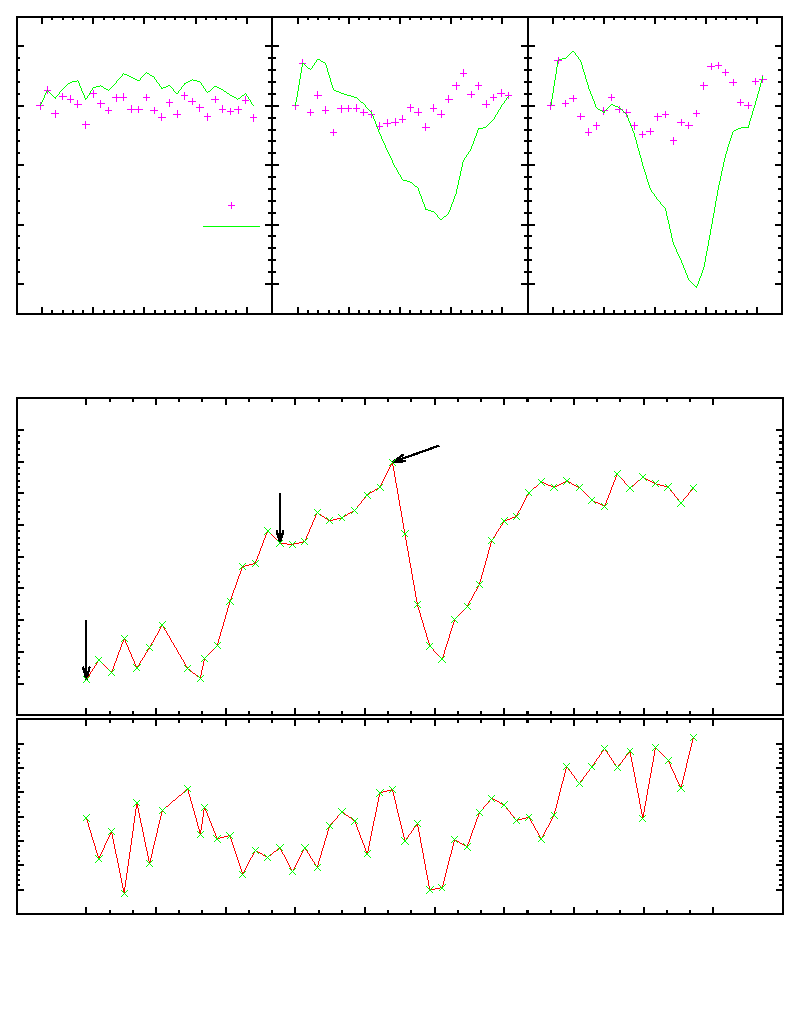
\includegraphics{linearitaet_verlauf}}%
    \gplfronttext
  \end{picture}%
\endgroup

	\caption[Linearitaet \textit{iScan}, zeitlicher Verlauf]{Abgebildet
	ist der zeitliche Verlauf des maximalen Scanfehler (oben) und der Abweichung
	des Paramters \lstinline|FSR| vom wahren FSR des \textit{iScans} (unten). Die
	Messung wurde unmittelbar nach Beendigung der Linearisierung aus Abb.
	\ref{fig:linearisierung_FSR_korr_01} gestartet.}
	\label{fig:linearitaet_verlauf}
\end{figure}
%TODO: !!!!!geschreibsel


Im nächsten Abschnitt soll nun überprüft werden, ob diese Werte zum fehlerfreien
Arbeiten genügen und den Performanceansprüchen bei der Frequenzverstimmung gerecht werden.

\subsection{Frequenzscans}\label{sec:frequenz_scans}

